% TEMPLATE for Usenix papers, specifically to meet requirements of
%  USENIX '05
% originally a template for producing IEEE-format articles using LaTeX.
%   written by Matthew Ward, CS Department, Worcester Polytechnic Institute.
% adapted by David Beazley for his excellent SWIG paper in Proceedings,
%   Tcl 96
% turned into a smartass generic template by De Clarke, with thanks to
%   both the above pioneers
% use at your own risk.  Complaints to /dev/null.
% make it two column with no page numbering, default is 10 point

% Munged by Fred Douglis <douglis@research.att.com> 10/97 to separate
% the .sty file from the LaTeX source template, so that people can
% more easily include the .sty file into an existing document.  Also
% changed to more closely follow the style guidelines as represented
% by the Word sample file. 
% This version uses the latex2e styles, not the very ancient 2.09 stuff.
\documentclass[letterpaper,twocolumn,10pt]{article}
\usepackage{usenix,epsfig,endnotes}
\usepackage[protrusion=true,expansion=true]{microtype}
\usepackage{color}
\usepackage{times}
\usepackage{url}
\usepackage{graphicx}
\usepackage{xspace}
\usepackage{textcomp}
\usepackage{subfig}

\newcommand{\JT} {JobTracker\xspace}
\newcommand{\TT} {TaskTracker\xspace}
\newcommand{\NN} {NameNode\xspace}
\newcommand{\DN} {DataNode\xspace}

% \newcommand{\paa}[1]{{\textcolor{blue}{#1 -- paa}}}
% \newcommand{\nrc}[1]{{\textcolor{green}{#1 -- nrc}}}
% \newcommand{\rcs}[1]{{\textcolor{red}{#1 -- rcs}}}
%\newcommand{\jmh}[1]{{\textcolor{red}{#1 -- jmh}}}

\begin{document}


%don't want date printed
\date{}

%make title bold and 14 pt font (Latex default is non-bold, 16 pt)
\title{\Large \bf MapReduce Online}

%for single author (just remove % characters)
\author{
{\rm Tyson Condie, Neil Conway, Peter Alvaro, Joseph M.\ Hellerstein}\\ UC Berkeley
\and
{\rm Khaled Elmeleegy, Russell Sears}\\ Yahoo! Research
}

\maketitle

\begin{abstract}
  MapReduce is a popular framework for data-intensive distributed computing of
  batch jobs. To simplify fault tolerance, many implementations of MapReduce
  \emph{materialize} the entire output of each map and reduce task before it can
  be consumed. In this paper, we propose a modified MapReduce architecture that
  allows data to be \emph{pipelined} between operators. This extends the
  MapReduce programming model beyond batch processing, and can reduce completion
  times and improve system utilization for batch jobs as well.  We present a
  modified version of the Hadoop MapReduce framework that supports \emph{online
    aggregation}, which allows users to see ``early returns'' from a job as it
  is being computed. Our Hadoop Online Prototype ({\em HOP}) also supports
  \emph{continuous queries}, which enable MapReduce programs to be written for
  applications such as event monitoring and stream processing. HOP retains the
  fault tolerance properties of Hadoop and can run unmodified user-defined
  MapReduce programs.
\end{abstract}

\section{Introduction} 
\label{sec:intro} 
Although distributed programming has become an essential and commonplace task,
it remains very challenging for most developers to write correct distributed
programs. The inherent difficulties of distributed computing---concurrency,
asynchrony, and partial failure---are exacerbated by the scale at which modern
distributed systems operate.

% remind reviewers that it's a database problem. can remove if accepted! 
Much of the discussion about distributed programming today revolves around data
management systems, and the tradeoffs between transactions and loose
consistency. Programmers using distributed transactions are relieved of
consistency concerns but often face significant performance and operational
challenges~\cite{Birman2009}. By contrast, programmers who use loosely
consistent systems can expect more predictable and low-latency performance, but
must reason explicitly about program correctness over inconsistent distributed
state.

In recent years there has been increased interest in techniques to help
programmers achieve correct program behavior without requiring strongly
consistent storage. This idea has been explored in two different frameworks,
\emph{Convergent Objects} and \emph{Monotonic Logic}.

\vspace{0.5em}\noindent
\textbf{Convergent Objects}: In this approach, a programmer writes encapsulated
object classes whose public methods guarantee certain properties regarding
message reordering and/or retry. For example, Statebox is an open-source library
that merges conflicting updates to data items in a key-value store; the user of
the library need only register commutative, idempotent merge
functions~\cite{statebox}. This approach has roots in research in
databases~\cite{Farrag1989,Garcia-Molina1983,Helland2009} and
groupware~\cite{Ellis1989,Sun1998}.  Shapiro et al.\ recently proposed a model
for these approaches called \emph{Conflict-Free Replicated Data Types} (CRDTs),
which formalizes these ideas in an algebraic framework~\cite{Shapiro2011b}.

The main problem with the CRDT approach is that its guarantees of correctness
are limited to an individual replicated data value, not to application logic in
general. For example, consider a distributed algorithmic trading service that
uses a CRDT to represent a mutable set \texttt{Portfolio}. Suppose one server
$M$ reads a local version of the set containing an element \texttt{BNNA} and
constructs an expected portfolio value $v = f(\mbox{\texttt{Portfolio}})$
derived from that version. Concurrently, \texttt{BNNA} is removed from the local
version of \texttt{Portfolio} at another server $N$. The CRDT can ensure that
$M$ and $N$ will eventually agree that \texttt{BNNA} is absent from the set, but
the application state at $M$ and $N$ may remain inconsistent unless the value
$v$ at $M$ is updated to reflect the removal of \texttt{BNNA}. Although the CRDT
maintains its own invariants, the programmer still bears the burden of ensuring
the consistency semantics of the entire program.

\vspace{0.5em} \noindent
\textbf{Monotonic Logic}: In recent work, we observed that the database theory
literature on non-monotonic logic provides a promising starting point for
reasoning about distributed consistency. Intuitively, a \emph{monotonic} program
computes more information over time---it never ``retracts'' an earlier
conclusion in the face of new information. We proposed the CALM
theorem~\cite{Hellerstein2010}, which established that all monotonic programs
are eventually consistent~\cite{Ameloot2011,dedalus-pods12-tr}. Monotonicity of
a Datalog-style program is straightforward to determine conservatively from
syntax, so the CALM theorem provides the basis for a simple analysis technique
for verifying the consistency of distributed programs~\cite{Alvaro2011}. We
realized the CALM analysis as part of Bloom, a Datalog-based DSL for distributed
programming~\cite{bloom}.

The original formulation of Bloom and CALM only validated consistency for programs that compute sets of facts that grow over time (``set monotonicity''); that is, ``growth'' is defined according to set containment. As a practical matter, this is overly conservative: several common distributed programming idioms that are monotonic do not satisfy syntactic monotonicity tests for Datalog. In particular, threshold tests over monotonic aggregate values (e.g., ``$\mathrm{max}(S) > k$'') and upward-moving mutable counters are both considered to be non-monotonic by the original CALM analysis.  As a result, the initial Bloom prototype advises the programmer to guard those constructs with strong consistency methods like Paxos~\cite{Lamport1998} or Two-Phase Commit. 

\subsection{A Hybrid Approach}
% The strengths and weaknesses of these two approaches appear complementary. CRDTs provide synchronization-free consistent objects, but cannot guarantee whole-program consistency. Bloom's CALM analysis guarantees whole-program consistency but is unable to verify a number of natural coordination-free mechanisms.
In this paper, we extend our previous work to accommodate the ideas underlying CRDTs. Instead of only allowing growth according to the set containment
partial order, we allow any user-defined partial order to be used.  
We do this by providing \emph{join semi-lattices} as a programming construct.
We give a
formal definition of this construct below, but the intuition is that the programmer provides a commutative, idempotent merge function (``least upper bound'')
that takes two input values and produces an output value that is not smaller
than either of the input values (according to the user's partial order). This
generalizes Bloom (and traditional Datalog), which assumes a fixed merge
function (set union) and partial order (set containment).
% Relate user-defined merge functions to merge functions in other contexts?
% (e.g., key-value store, COPS, Piccolo)

% Explain how lattices generalize monotonic datalog
It is attractive to incorporate join semi-lattices into logic programming,  but doing so raises challenges in language design, consistency analysis and efficient execution.  In this paper, we make the following contributions:
\begin{enumerate}
% \item
%   We present \baselang, a variant of Datalog that is defined over lattices. We
%   define a model-theoretic semantics for \baselang, and show that \baselang
%   generalizes Datalog.

\item
  We introduce \lang, an extension of Bloom that supports lattices. We detail
  the builtin lattice types provided by \lang and show how developers can
  define new lattices.
  
\item 
  We provide interfaces for consistency-preserving mappings across lattices via
  \emph{morphisms} and \emph{monotonic functions}.  This is critical for \lang
  and forms a useful extension to the CRDT framework as well.

\item 
  We generalize the CALM analysis to programs that contain both lattices and
  set-oriented collections, and show how lattices can be used to prove the
  confluence of several common distributed design patterns that were regarded as
  non-monotonic in Bloom. % XXX: revisit this

\item
  For efficient execution, we show how to extend the standard Datalog semi-naive
  evaluation scheme~\cite{Balbin1987} to support both lattices and traditional
  database relations. We also describe how an existing Datalog engine can be
  extended to support lattices with relatively minor changes.

\item
  Finally, we demonstrate the usefulness of lattices with two case studies.
  First we revisit the simple e-commerce scenario presented in Alvaro et al., in
  which clients interact with a replicated shopping cart
  service~\cite{Alvaro2011}. We show how \lang can be used to make the
  ``checkout'' operation monotonic, despite the fact that it requires
  aggregating over a distributed data set.

  Second, we use \lang to implement vector clocks and causal delivery, two
  standard building blocks for distributed programming. We show how both
  algorithms can be realized as monotonic \lang programs that are concise and
  readable.
\end{enumerate}

\section{Background}
\label{sec:background}

% XXX: should this be a distributed example?
\begin{figure}[t]
\begin{scriptsize}
\begin{lstlisting}
class ShortestPaths
  include Bud

  state do
    table :link, [:from, :to] => [:cost] (*\label{line:spaths-ddl}*)
    scratch :path, [:from, :to, :next_hop, :cost]
    scratch :min_cost, [:from, :to] => [:cost]
  end

  bloom do
    path <= link {|l| [l.from, l.to, l.to, l.cost]} (*\label{line:spaths-proj}*)
    path <= (link*path).pairs(:to => :from) do |l,p| (*\label{line:spaths-join-start}*)
      [l.from, p.to, l.to, l.cost + p.cost]
    end (*\label{line:spaths-join-end}*)

    min_cost <= path.group([:from, :to], min(:cost)) (*\label{line:spaths-group}*)
  end
end
\end{lstlisting}
\end{scriptsize}
\caption{All-pairs shortest paths in Bloom.}
\label{fig:bloom-spaths}
\end{figure}

In this section, we review the Bloom programming language and the CALM program
analysis.  We highlight a simple distributed program for which the CALM analysis
yields unsatisfactory results.

\subsection{Bloom}
\label{sec:bg-bloom}

Bloom is a Datalog-based domain-specific language (DSL) for distributed
programming~\cite{Alvaro2011,bloom}. The state of a Bloom program is represented
using \emph{collections} and computation is expressed as a bundle of declarative
\emph{statements}.  An instance of a Bloom program performs computation by
evaluating its statements over the contents of its local database. Bloom
instances communicate via asynchronous messaging, as described further below.

An instance of a Bloom program proceeds through a series of \emph{timesteps},
each containing three phases.\footnote{There is a precise declarative semantics
  for Bloom~\cite{dedalus}, but we describe the language operationally for the
  sake of exposition.} In the first phase, inbound events (e.g., network
messages) are received and represented as facts in collections. In the second
phase, the program's statements are evaluated over local state to compute all
the additional facts that can be derived from the current collection
contents. In some cases (described below), a derived fact is intended to achieve
a ``side effect,'' such as modifying local state or sending a network message.
These effects are deferred during the second phase of the timestep; the third
phase is devoted to carrying them out.

The initial implementation of Bloom, called \emph{Bud}, allows Bloom logic to be
embedded inside a Ruby program. Figure~\ref{fig:bloom-spaths} shows a Bloom
program represented as an annotated Ruby class. A small amount of imperative
Ruby code is needed to instantiate the Bloom program and begin executing it;
more details are available on the Bloom language website~\cite{bloom}.

\subsubsection{Data model}
\begin{table}[t]
\begin{tabular}{|l|p{2.32in}|}
\hline
\textbf{Name} & \textbf{Behavior }\\
\hline
\texttt{table} & Persistent storage.\\
\texttt{scratch} & Transient storage.\\
\texttt{channel} & Asynchronous communication. A fact derived into a \texttt{channel} appears in the
database of a remote Bloom instance at a non-deterministic future time.\\
\texttt{periodic} & Interface to the system clock.\\
\texttt{interface} & Interface point between software modules.\\
\hline
\end{tabular}
\caption{Bloom collection types.}
\label{tbl:bloom-collections}
\end{table}

The Bloom data model is based on \emph{collections}.  A collection is an
unordered set of \emph{facts}, akin to a relation in Datalog. The Bud prototype
adopts the Ruby type system rather than inventing its own; hence, a fact in Bud
is just an array of Ruby objects. Each collection has a \emph{schema}, which
declares the structure (column names) of the facts in the collection. A subset
of the columns in a collection form its \emph{key}: as in the relational model,
the key columns functionally determine the remaining columns. The collections
used by a Bloom program are declared in a \texttt{state} block. For example,
line~\ref{line:spaths-ddl} of Figure~\ref{fig:bloom-spaths} declares a
collection named \texttt{link} with three columns, two of which form the
collection's key. Ruby is a dynamically typed language, so keys and values in
Bud can hold arbitrary Ruby objects.

Bloom provides five collection types to represent different kinds of state
(Table~\ref{tbl:bloom-collections}). A \texttt{table} stores persistent data: if
a fact appears in a table, it remains in the table in future timesteps (unless it
is explicitly removed). A \texttt{scratch} contains transient data---the content
of scratch collections is emptied at the start of each timestep. Scratches are
akin to SQL views: they are often useful as a way to name intermediate results
or as a ``macro'' construct to enable code reuse. The \texttt{channel}
collection type enables communication between Bloom instances. The schema of a
channel has a distinguished \emph{location specifier} column (prefixed with
``\texttt{@}''); when a fact is derived for a channel collection, it appears in
the database of the Bloom instance at the address given by the location
specifier. The \texttt{periodic} and \texttt{interface} collection types do not
arise in our discussion in this paper; the interested reader is referred to the
Bloom website~\cite{bloom}.

\subsubsection{Statements}
\begin{table}
\begin{tabular}{|c|l|p{1.85in}|}
\hline
\textbf{Op} & \textbf{Name} & \textbf{Meaning} \\
\hline
\verb|<=| & \emph{merge} & lhs includes the content of rhs in the
current timestep \\
\hline
\verb|<+| & \emph{deferred merge} & lhs will include the content of rhs in the
next timestep \\
\hline
\verb|<-| & \emph{deferred delete} & lhs will not include the content of rhs
in the next timestep \\
\hline
\verb|<~| & \emph{async merge} & (remote) lhs will include the content of the
rhs at some non-deterministic future timestep\\
\hline
\end{tabular}
\caption{Bloom operators.}
\label{tbl:bloom-ops}
\end{table}

Each Bloom statement has one or more input collections and a single output
collection.  A statement takes the form: \\ \noindent
\mbox{\hspace{0.25in}\emph{$<$collection-identifier$>$ $<$op$>$
    $<$collection-expression$>$}}\\ \noindent
The left-hand side (lhs) is the name of the output collection and the right-hand
side (rhs) is an expression that produces a collection.  A statement defines how
the contents of the input collections should be transformed before being
included (via set union) in the output collection. Bloom allows the usual
relational operators to be used on the rhs (selection, projection, join,
grouping, aggregation, and negation), although it adopts a syntax intended to be
more familiar to imperative programmers. In Figure~\ref{fig:bloom-spaths},
line~\ref{line:spaths-proj} demonstrates projection,
lines~\ref{line:spaths-join-start}--\ref{line:spaths-join-end} perform a join
between \texttt{link} and \texttt{path} using the join predicate
\verb+link.to = path.from+ followed by a projection to four attributes, and
line~\ref{line:spaths-group} demonstrates grouping and aggregation. Bloom
statements appear in one or more \texttt{bloom} blocks. A Bloom program can also
include a \texttt{bootstrap} block, which contains statements that are evaluated
only once when a Bloom instance starts executing. \texttt{bootstrap} blocks are
typically used for initialization or configuration data.

Bloom provides several operators that determine \emph{when} the rhs will be
merged into the lhs (Table~\ref{tbl:bloom-ops}). The \verb|<=| operator performs
standard logical deduction: that is, the lhs and rhs are true at the same
timestep. The \verb|<+| and \verb|<-| operators indicate that facts will be
added or removed, respectively, from the lhs collection at the beginning of the
\emph{next} timestep. The \verb+<~+ operator specifies that the rhs will be merged into
the lhs collection at some non-deterministic future time. The lhs of a statement
that uses \verb+<~+ must be a channel; the \verb+<~+ operator captures
asynchronous messaging.

% XXX: does this need to be said?
Bloom allows recursion---i.e., the rhs of a statement can reference the lhs
collection, either directly or indirectly. As in Datalog, certain constraints
must be adopted to ensure that programs with recursive statements have a
sensible interpretation. For deductive statements (\verb+<=+ operator), we
require that programs be \emph{syntactically stratified}~\cite{Apt1988}: cycles
through negation or aggregation are not allowed (unless they contain a deferred
or asynchronous operator)~\cite{dedalus}.

\subsection{CALM analysis}
\label{sec:bg-calm}

Work on deductive databases has long drawn a distinction between
\emph{monotonic} and \emph{non-monotonic} logic programs. Intuitively, a
monotonic program only computes more information over time---it will never
``retract'' a previous conclusion in the face of new evidence.  In Bloom (and
Datalog), a simple conservative test for monotonicity is based on program
syntax: selection, projection, and join are monotonic, while aggregation and
negation are not.

The CALM theorem connects the theory of monotonic logic with the practical
problem of distributed consistency~\cite{Alvaro2011,Hellerstein2010}.  All
monotonic programs are ``eventually consistent'' or \emph{confluent}: for any
given input, all program executions result in the same final state regardless of
network non-determinism~\cite{Ameloot2011,dedalus-confluence}.  Hence, monotonic
logic is a useful building block for loosely consistent distributed programming.

According to the CALM theorem, distributed inconsistency may only occur at
\emph{points of order}: program locations where the output of an asynchronously
derived value is consumed by a non-monotonic operator.  This is because
asynchronous messaging results in non-deterministic arrival order, and
non-monotonic operators may be produce different conclusions when evaluated over
different subsets of their inputs.  For example, consider a Bloom program in
which collections $A$ and $B$ are fed by asynchronous channels and the program
sends a message whenever an element of $A$ arrives that is not in $B$. This
program is non-monotonic and exhibits non-confluent behavior: the messages sent
by the program will depend on the order in which the elements of $A$ and $B$
arrive.

We have implemented a conservative static program analysis in Bloom that follows
directly from the CALM theorem.  Programs that are free from non-monotonic
constructs are ``blessed'' as confluent: producing the same output on different
runs or converging to the same state on multiple distributed replicas.
Otherwise, programs are flagged as potentially inconsistent.  To achieve
consistency, the programmer either needs to rewrite their program to avoid the
use of non-monotonicity or introduce a coordination protocol to ensure that a
consistent ordering is agreed upon. Coordination protocols incur additional
latency and reduce availability in the event of network partitions, so in this
paper we focus on coordination-free designs---that is, monotonic programs.

\subsubsection{Limitations of set monotonicity}
The original formulation of the CALM theorem considered only programs that
compute more facts over time---that is, programs whose output \emph{sets} grow
monotonically. Many distributed protocols make progress over time, but their
notion of ``progress'' is often difficult to represent as a growing set of
facts. For example, consider the Bloom program in
Figure~\ref{fig:bloom-nm-quorum}. This program receives votes from a client
program (not shown) via the \texttt{vote\_chn} channel. Once at least
\texttt{QUORUM\_SIZE} votes have been received, a message is sent to a remote
node to indicate that quorum has been reached
(line~\ref{line:bloom-quorum-msg}). This program resembles a ``quorum vote''
subroutine that might be used by an implementation of Paxos~\cite{Lamport1998}
or quorum replication~\cite{Gifford1979}.

It is easy to see that this program makes progress in a semantically monotonic
fashion: the set of received votes grows and the size of the \texttt{votes}
collection can only increase, so once a quorum has been reached it will never be
retracted. Unfortunately, the current CALM analysis would regard this program as
non-monotonic because it contains aggregation (the grouping operation on
line~\ref{line:bloom-nm-quorum}).

To solve this problem, we need to introduce a notion of program values that
``grow'' according to a partial order other than set containment. We do this by
extending Bloom to operate over arbitrary lattices, rather than just the
set lattice.

%  We present a
% complete language in the following section, but the intuition can be observed in
% Figure~\ref{fig:lattice-quorum}. Votes are accumulated into a set lattice
% (line~\ref{line:quorum-set-accum}), but the size of the set is represented as an
% \texttt{lmax} lattice (line~\ref{line:quorum-lmax}): that is, a number that
% never decreases. Hence, a threshold test ``$\ge k$'' on an \texttt{lmax} lattice
% is monotonic map onto the boolean lattice: that is, the \texttt{quorum\_done}
% predicate goes from false to true (and then remains true).

\begin{figure}[t]
\begin{scriptsize}
\begin{lstlisting}
QUORUM_SIZE = 5
RESULT_ADDR = "example.org"

class QuorumVote
  include Bud

  state do
    channel :vote_chn, [:@addr, :voter_id]
    channel :result_chn, [:@addr]
    table   :votes, [:voter_id]
    scratch :cnt, [] => [:cnt]
  end

  bloom do
    votes      <= vote_chn {|v| [v.voter_id]}
    cnt        <= votes.group(nil, count(:voter_id)) (*\label{line:bloom-nm-quorum}*)
    result_chn <~ cnt {|c| [RESULT_ADDR] if c >= QUORUM_SIZE} (*\label{line:bloom-quorum-msg}*)
  end
end
\end{lstlisting}
\end{scriptsize}
\caption{A non-monotonic Bloom program that waits for a quorum of votes to be received.}
\label{fig:bloom-nm-quorum}
\end{figure}

\section{Pipelined MapReduce}
\label{sec:pipelining}
%\begin{figure}[t]
%  \centering
%        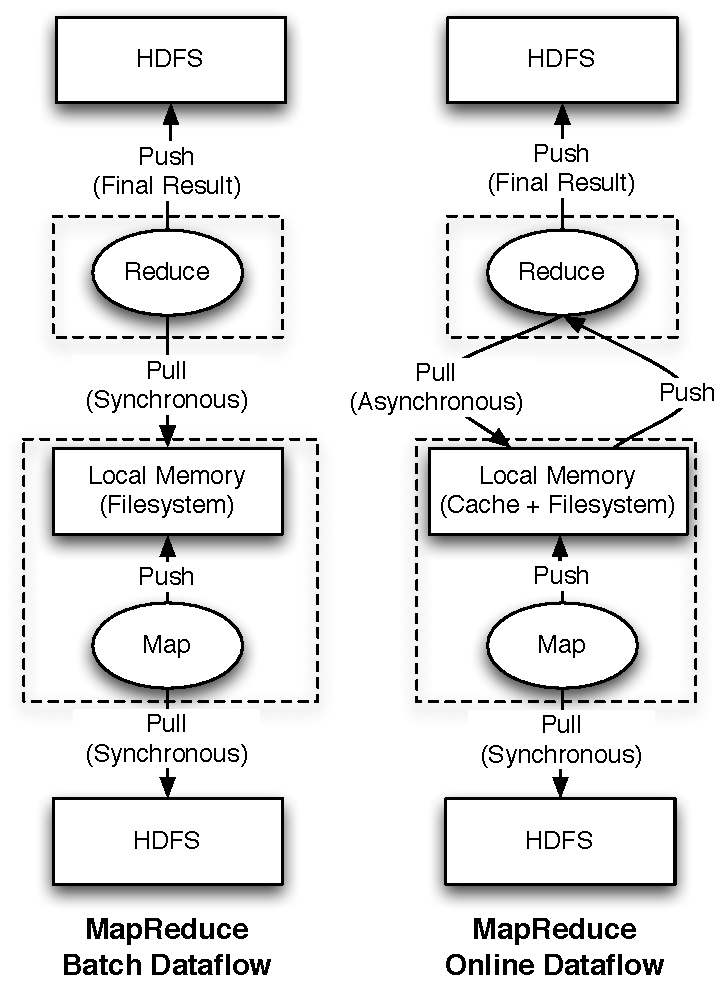
\includegraphics[width=0.90\linewidth]{figures/dataflow_arch.pdf}
%       \caption{Hadoop dataflow for batch (left) and pipelined (right) processing of MapReduce computations.}
%        \label{fig:pipeline}
%\end{figure}

In this section we discuss our extensions to Hadoop to support pipelining
between tasks (Section~\ref{sec:intra-pipe}) and between jobs
(Section~\ref{sec:inter-pipe}).  We describe how our design supports fault
tolerance (Section~\ref{sec:ft}), and discuss the interaction between pipelining
and task scheduling (Section~\ref{sec:pipeline-sched}).  Our focus here is on
batch-processing workloads; we discuss online aggregation and continuous queries
in Section~\ref{sec:online} and Section~\ref{sec:continuous}. We defer
performance results to Section~\ref{sec:perf}.

%Figure~\ref{fig:pipeline} depicts the dataflow of two MapReduce
%implementations. The dataflow on the left corresponds to the output
%materialization approach used by regular Hadoop; the dataflow on the right
%allows pipelining. In the remainder of this section, we present our design and
%implementation for the pipelined Hadoop dataflow. We describe how our design
%supports fault tolerance (Section~\ref{sec:ft}), and discuss the interaction
%between pipelining and task scheduling (Section~\ref{sec:pipeline-sched}).

\subsection{Pipelining Within A Job}
\label{sec:intra-pipe}
As described in Section~\ref{sec:reducetask}, reduce tasks
traditionally issue HTTP requests to \emph{pull} their output from
each {\TT}. This means that map task execution is completely decoupled
from reduce task execution. To support pipelining, we modified the map
task to instead \emph{push} data to reducers as it is produced. To
give an intuition for how this works, we begin by describing a
straightforward pipelining design, and then discuss the changes we
had to make to achieve good performance.

\subsubsection{Na\"{\i}ve Pipelining}
\label{sec:naive}
In our na\"{\i}ve implementation, we modified Hadoop to send data directly from
map to reduce tasks. When a client submits a new job to Hadoop, the {\JT}
assigns the map and reduce tasks associated with the job to the available {\TT}
slots. For purposes of discussion, we assume that there are enough free slots to
assign all the tasks for each job. We modified Hadoop so that each reduce task
contacts every map task upon initiation of the job, and opens a TCP socket which
will be used to pipeline the output of the map function. As each map output
record is produced, the mapper determines which partition (reduce task) the
record should be sent to, and immediately sends it via the appropriate socket.

A reduce task accepts the pipelined data it receives from each map task and
stores it in an in-memory buffer, spilling sorted runs of the buffer to disk as
needed. Once the reduce task learns that every map task has completed, it
performs a final merge of all the sorted runs and applies the user-defined
reduce function as normal.

\subsubsection{Refinements}
\label{sec:pipe-refine}
While the algorithm described above is straightforward, it suffers
from several practical problems. First, it is possible that there will
not be enough slots available to schedule every task in a new
job. Opening a socket between every map and reduce task also requires
a large number of TCP connections. A simple tweak to the na\"{\i}ve
design solves both problems: if a reduce task has not yet been
scheduled, any map tasks that produce records for that partition
simply write them to disk. Once the reduce task is assigned a slot, it
can then pull the records from the map task, as in regular Hadoop.  To
reduce the number of concurrent TCP connections, each reducer can be
configured to pipeline data from a bounded number of mappers at once; the
reducer will pull data from the remaining map tasks in the traditional
Hadoop manner.

% nrc: Not interesting?
Our initial pipelining implementation suffered from a second problem: the map
function was invoked by the same thread that wrote output records to the
pipeline sockets. This meant that if a network I/O operation blocked (e.g.,
because the reducer was over-utilized), the mapper was prevented from doing
useful work. Pipeline stalls should not prevent a map task from making
progress---especially since, once a task has completed, it frees a {\TT} slot
to be used for other purposes. We solved this problem by running the map
function in a separate thread that stores its output in an in-memory buffer, and
then having another thread periodically send the contents of the buffer to the
connected reducers.

\subsubsection{Granularity of Map Output}
\label{sec:mapout}

Another problem with the na\"{\i}ve design is that it eagerly sends
each record as soon as it is produced, which prevents the use of
map-side combiners. Imagine a job where the reduce key has few
distinct values (e.g., gender), and the reduce applies an aggregate
function (e.g., count). As discussed in Section~\ref{sec:progmodel},
combiners allow map-side ``pre-aggregation'': by applying a
reduce-like function to each distinct key at the mapper, network
traffic can often be substantially reduced. Eagerly pipelining each
record as it is produced prevents the use of map-side combiners.

A related problem is that eager pipelining moves some of the sorting
work from the mapper to the reducer. Recall that in the blocking
architecture, map tasks generate sorted spill files: all the reduce
task must do is merge together the pre-sorted map output for each
partition. In the na\"{\i}ve pipelining design, map tasks send output
records in the order in which they are generated, so the reducer must
perform a full external sort. Because the number of map tasks
typically far exceeds the number of reduces~\cite{mapreduce-osdi},
moving more work to the reducer increased response time in our
experiments.

We addressed these issues by modifying the in-memory buffer design described in
Section~\ref{sec:pipe-refine}. Instead of sending the buffer contents to
reducers directly, we wait for the buffer to grow to a threshold
size. The mapper then applies the combiner function, sorts the output by
partition and reduce key, and writes the buffer to disk using the spill file
format described in Section~\ref{sec:maptask}.

Next, we arranged for the {\TT} at each node to handle pipelining data to reduce
tasks. Map tasks register spill files with the {\TT} via RPCs. If the reducers
are able to keep up with the production of map outputs and the network is not a
bottleneck, a spill file will be sent to a reducer soon after it has been
produced (in which case, the spill file is likely still resident in the map
machine's kernel buffer cache). However, if a reducer begins to fall behind, the
number of unsent spill files will grow.

When a map task generates a new spill file, it first queries the {\TT} for the
number of unsent spill files. If this number grows beyond a certain threshold
(two unsent spill files in our experiments), the map task does not immediately
register the new spill file with the {\TT}. Instead, the mapper will accumulate
multiple spill files. Once the queue of unsent spill files falls below the
threshold, the map task merges and combines the accumulated spill files into a
single file, and then resumes registering its output with the {\TT}. This simple
flow control mechanism has the effect of \emph{adaptively} moving load from the
reducer to the mapper or vice versa, depending on which node is the current
bottleneck.

A similar mechanism is also used to control how aggressively the combiner
function is applied. The map task records the ratio between the input and output
data sizes whenever it invokes the combiner function. If the combiner is
effective at reducing data volumes, the map task accumulates more spill files
(and applies the combiner function to all of them) before registering that
output with the {\TT} for pipelining.\footnote{Our current prototype uses a
  simple heuristic: if the combiner reduces data volume by $\frac{1}{k}$ on
  average, we wait until $k$ spill files have accumulated before registering
  them with the {\TT}. A better heuristic would also account for the computational
  cost of applying the combiner function.}

The connection between pipelining and adaptive query processing techniques has
been observed elsewhere (e.g.,~\cite{eddies}). The adaptive scheme outlined
above is relatively simple, but we believe that adapting to feedback along
pipelines has the potential to significantly improve the utilization of
MapReduce clusters.

\subsection{Pipelining Between Jobs}
\label{sec:inter-pipe}

Many practical computations cannot be expressed as a single MapReduce job, and
the outputs of higher-level languages like Pig~\cite{pig} typically involve
multiple jobs.  In the traditional Hadoop architecture, the output of each job
is written to HDFS in the reduce step and then immediately read back from HDFS
by the map step of the next job. Furthermore, the {\JT} cannot schedule a
consumer job until the producer job has completed, because scheduling a map task
requires knowing the HDFS block locations of the map's input split.

In our modified version of Hadoop, the reduce tasks of one job can optionally
pipeline their output directly to the map tasks of the next job, sidestepping
the need for expensive fault-tolerant storage in HDFS for what amounts to a
temporary file. Unfortunately, the computation of the reduce function from the
previous job and the map function of the next job cannot be overlapped: the
final result of the reduce step cannot be produced until all map tasks have
completed, which prevents effective pipelining. However, in the next sections we
describe how online aggregation and continuous query pipelines can publish
``snapshot'' outputs that can indeed pipeline between jobs.

\subsection{Fault Tolerance}
\label{sec:ft}

% nrc: (1) Quantify the overhead added by tracking map task origin (2)
% Did we implement the "don't rerun map task from scratch" idea?

Our pipelined Hadoop implementation is robust to the failure of both
map and reduce tasks. To recover from map task failures, we added
bookkeeping to the reduce task to record which map task produced each
pipelined spill file. To simplify fault tolerance, the reducer treats
the output of a pipelined map task as ``tentative'' until the {\JT}
informs the reducer that the map task has committed successfully. The
reducer can merge together spill files generated by the same
uncommitted mapper, but will not combine those spill files with the
output of other map tasks until it has been notified that the map task
has committed. Thus, if a map task fails, each reduce task can ignore
any tentative spill files produced by the failed map attempt. The
{\JT} will take care of scheduling a new map task attempt, as in stock
Hadoop. 

If a reduce task fails and a new copy of the task is started, the new
reduce instance must be sent all the input data that was sent to the
failed reduce attempt. If map tasks operated in a purely pipelined
fashion and discarded their output after sending it to a reducer, this
would be difficult. Therefore, map tasks retain their output data on
the local disk for the complete job duration. This allows the map's output to be 
reproduced if any reduce tasks fail. For batch jobs, the key advantage of our architecture is
that reducers are not blocked waiting for the complete output of the
task to be written to disk.

Our technique for recovering from map task failure is straightforward, but
places a minor limit on the reducer's ability to merge spill files. To avoid
this, we envision introducing a ``checkpoint'' concept: as a map task runs, it
will periodically notify the {\JT} that it has reached offset $x$ in its input
split. The {\JT} will notify any connected reducers; map task output that was
produced before offset $x$ can then be merged by reducers with other map task
output as normal. To avoid duplicate results, if the map task fails, the new map
task attempt resumes reading its input at offset $x$. This technique would also
reduce the amount of redundant work done after a map task failure or during
speculative execution of ``backup'' tasks~\cite{mapreduce-osdi}.

\subsection{Task Scheduling}
\label{sec:pipeline-sched}

The Hadoop {\JT} had to be retrofitted to support pipelining between jobs. In
regular Hadoop, job are submitted one at a time; a job that consumes the output
of one or more other jobs cannot be submitted until the producer jobs have
completed. To address this, we modified the Hadoop job submission interface to
accept a list of jobs, where each job in the list depends on the job before
it. The client interface traverses this list, annotating each job with the
identifier of the job that it depends on. The {\JT} looks for this annotation
and co-schedules jobs with their dependencies, giving slot preference to
``upstream'' jobs over the ``downstream'' jobs they feed.  As we note in
Section~\ref{sec:concl}, there are many interesting options for scheduling
pipelines or even DAGs of such jobs that we plan to investigate in future.

\section{Online Aggregation}
\label{sec:online}

Although MapReduce was originally designed as a batch-oriented system,
it is often used for interactive data analysis: a user submits a job
to extract information from a data set, and then waits to view the
results before proceeding with the next step in the data analysis
process. This trend has accelerated with the development of high-level
query languages that are executed as MapReduce jobs, such as
Hive~\cite{hive}, Pig~\cite{pig}, and Sawzall~\cite{sawzall}.

Traditional MapReduce implementations provide a poor interface for interactive
data analysis, because they do not emit any output until the job has been
executed to completion. In many cases, an interactive user would prefer a
``quick and dirty'' approximation over a correct answer that takes much longer
to compute. In the database literature, online aggregation has been proposed to
address this problem~\cite{onlineagg}, but the batch-oriented nature of
traditional MapReduce implementations makes these techniques difficult to
apply. In this section, we show how we extended our pipelined Hadoop
implementation to support online aggregation within a single job
(Section~\ref{sec:online-single}) and between multiple jobs
(Section~\ref{sec:online-multi}). In Section~\ref{sec:online-eval}, we evaluate
online aggregation on two different data sets, and show that it can yield an
accurate approximate answer long before the job has finished executing.

\subsection{Single-Job Online Aggregation}
\label{sec:online-single}

In HOP, the data records produced by map tasks are sent to reduce tasks shortly
after each record is generated. However, to produce the final output of the job,
the reduce function cannot be invoked until the entire output of every map task
has been produced. We can support online aggregation by simply applying the
reduce function to the data that a reduce task has received so far. We call the
output of such an intermediate reduce operation a \emph{snapshot}.

Users would like to know how accurate a snapshot is: that is, how
closely a snapshot resembles the final output of the job. Accuracy
estimation is a hard problem even for simple SQL queries~\cite{dbo}, 
and particularly hard for jobs where the map and reduce
functions are opaque user-defined code. Hence, we report job \emph{progress}, not
accuracy: we leave it to the user (or their MapReduce code) to correlate
progress to a formal notion of accuracy.  We give a simple progress metric below.

Snapshots are computed periodically, as new data arrives at each reducer. The
user specifies how often snapshots should be computed, using the progress metric
as the unit of measure. For example, a user can request that a snapshot be
computed when 25\%, 50\%, and 75\% of the input has been seen. The user may also
specify whether to include data from tentative (unfinished) map tasks. This
option does not affect the fault tolerance design described in
Section~\ref{sec:ft}. In the current prototype, each snapshot is stored in a
directory on HDFS\@. The name of the directory includes the progress value
associated with the snapshot. Each reduce task runs independently, and at a
different rate. Once a reduce task has made sufficient progress, it writes a
snapshot to a temporary directory on HDFS, and then atomically renames it to the
appropriate location.

Applications can consume snapshots by polling HDFS in a predictable
location. An application knows that a given snapshot has been
completed when every reduce task has written a file to the snapshot
directory.  Atomic rename is used to avoid applications mistakenly
reading incomplete snapshot files.

Note that if there are not enough free slots to allow all the reduce tasks in a
job to be scheduled, snapshots will not be available for reduce tasks that are
still waiting to be executed. The user can detect this situation (e.g.,\ by
checking for the expected number of files in the HDFS snapshot directory), so
there is no risk of incorrect data, but the usefulness of online aggregation
will be reduced. In the current prototype, we manually configured the cluster to
avoid this scenario. The system could also be enhanced to avoid this pitfall
entirely by optionally waiting to execute an online aggregation job until there
are enough reduce slots available.

\subsubsection{Progress Metric}
\label{sec:online-metric}
Hadoop provides support for monitoring the progress of task
executions. As each map task executes, it is assigned a \emph{progress
  score} in the range [0,1], based on how much of its input the map
task has consumed. We reused this feature to determine how much
progress is represented by the current input to a reduce task, and
hence to decide when a new snapshot should be taken.

First, we modified the spill file format depicted in
Figure~\ref{fig:mapoutput} to include the map's current progress
score. When a partition in a spill file is sent to a reducer, the
spill file's progress score is also included. To compute the progress
score for a snapshot, we take the average of the progress scores
associated with each spill file used to produce the snapshot.

Note that it is possible that a map task might not have pipelined
\emph{any} output to a reduce task, either because the map task has
not been scheduled yet (there are no free {\TT} slots), the map tasks does 
not produce any output for the given reduce task, or because the reduce task has 
been configured to only pipeline data from at most $k$ map tasks concurrently. 
To account for this, we need to scale the progress metric to reflect the portion 
of the map tasks that a reduce task has pipelined data from: if a reducer is 
connected to $\frac{1}{n}$ of the total number of map tasks in the job, we divide
the average progress score by $n$.

This progress metric could easily be made more sophisticated: for example, an
improved metric might include the selectivity ($|output|/|input|$) of each map task, the
statistical distribution of the map task's output, and the effectiveness of each
map task's combine function, if any. 
% We also assume that each map task
% constitutes a random sample from the input file; otherwise, the scale
% factor we use to account for unavailable map input will introduce
% bias. 
Although we have found our simple progress metric to be
sufficient for most experiments we describe below, this clearly
represents an opportunity for future work.

\subsection{Multi-Job Online Aggregation}
\label{sec:online-multi}

Online aggregation is particularly useful when applied to a long-running
analysis task composed of multiple MapReduce jobs.  As described in
Section~\ref{sec:inter-pipe}, our version of Hadoop allows the output of a
reduce task to be sent directly to map tasks. This feature can be used to
support online aggregation for a sequence of jobs.

Suppose that $j_1$ and $j_2$ are two MapReduce jobs, and $j_2$
consumes the output of $j_1$. When $j_1$'s reducers compute a snapshot
to perform online aggregation, that snapshot is written to HDFS, and
also sent directly to the map tasks of $j_2$. The map and reduce steps
for $j_2$ are then computed as normal, to produce a snapshot of
$j_2$'s output. This process can then be continued to support online
aggregation for an arbitrarily long sequence of jobs.
  
Unfortunately, inter-job online aggregation has some drawbacks. First,
the output of a reduce function is not ``monotonic'': the output of a
reduce function on the first 50\% of the input data may not be
obviously related to the output of the reduce function on the first
25\%. Thus, as new snapshots are produced by $j_1$, $j_2$ must be
recomputed from scratch using the new snapshot. As with inter-job
pipelining (Section~\ref{sec:inter-pipe}), this could be optimized for
reduce functions that are declared to be distributive or algebraic
aggregates~\cite{datacube}.

%%Fault tolerance with inter-job online aggregation is handled in three
%%cases. 
To support fault tolerance for multi-job online aggregation, we consider three
cases. Tasks that fail in $j_1$ recover as described in Section~\ref{sec:ft}.
If a task in $j_2$ fails, the system simply restarts the failed task. Since
subsequent snapshots produced by $j_1$ are taken from a superset of the mapper
output in $j_1$, the next snapshot received by the restarted reduce task in
$j_2$ will have a higher progress score. To handle failures in $j_1$, tasks in
$j_2$ cache the most recent snapshot received by $j_1$, and replace it when they
receive a new snapshot with a higher progress metric. If tasks from both jobs
fail, a new task in $j_2$ recovers the most recent snapshot from $j_1$ that was
stored in HDFS and then wait for snapshots with a higher progress score.

%Figure~\ref{fig:snapshot} depicts an inter-job dataflow for batch
%mode (left) and a dataflow that supports online aggregation
%(right). The batch mode forces jobs to read the final output of other
%jobs from HDFS\@.  

%%We support not only reading snapshots from HDFS but
%%also pipelining snapshots directly to jobs that request them. 
% In addition to reading snapshots from HDFS, we support pipelining
% snapshots directly to the jobs that request them.
% This is
% supported via an asynchronous request call interface exported by
% each reduce task, through which map tasks from other jobs can request
% snapshots and even the final output. The final output is concurrently
% written to HDFS for fault tolerance, unless otherwise specified in the
% configuration of the job.
  
% nrc: Discuss progress metric for inter-job OA
  
\subsection{Evaluation}
\label{sec:online-eval}

\begin{figure}
  \centering
    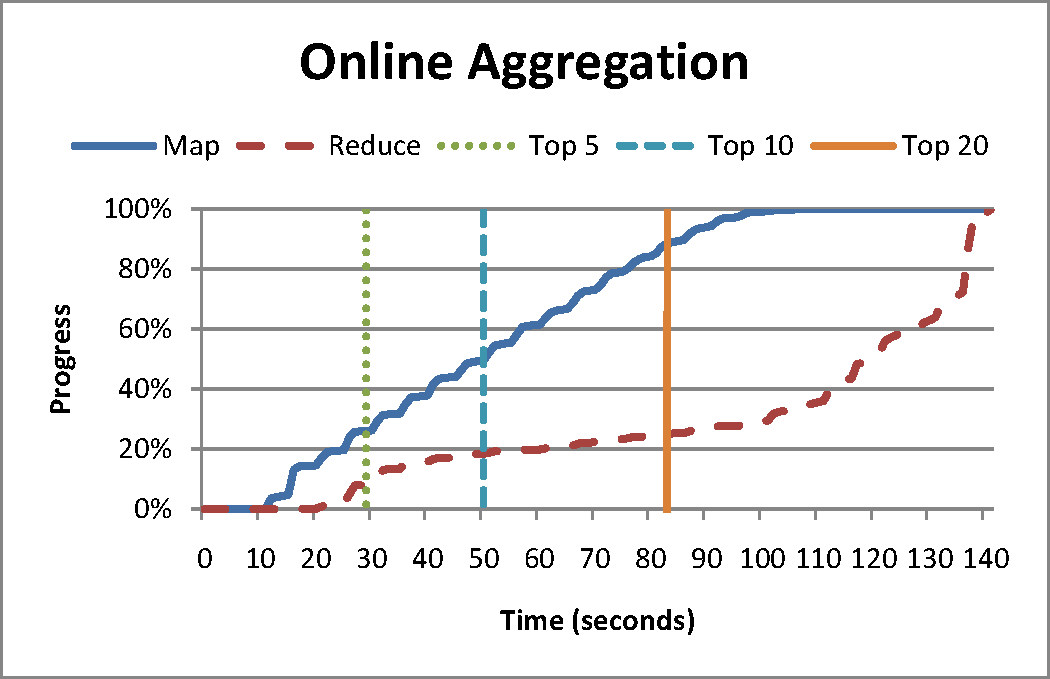
\includegraphics[width=0.95\linewidth]{eval/top100_online_wiki}
    \caption{Top-100 query over 5.5GB of Wikipedia article text. The vertical
      lines describe the increasing accuracy of the approximate answers produced
      by online aggregation.}
\label{fig:topkonlinewiki}
\vspace{-10pt}
\end{figure}

To evaluate the effectiveness of online aggregation, we performed two
experiments on Amazon EC2 using different data sets and query workloads. In our
first experiment, we wrote a ``Top-$K$'' query using two MapReduce jobs: the
first job counts the frequency of each word and the second job selects the $K$
most frequent words. We ran this workload on 5.5GB of Wikipedia article text
stored in HDFS, using a 128MB block size. We used a 60-node EC2 cluster; each
node was a ``high-CPU medium'' EC2 instance with 1.7GB of RAM and 2 virtual
cores. A virtual core is the equivalent of a 2007-era 2.5Ghz Intel Xeon
processor. A single EC2 node executed the Hadoop \JT\ and the HDFS \NN, while
the remaining nodes served as slaves for running the {\TT}s and HDFS {\DN}s.

% To evaluate inter-job dataflow with online aggregation we wrote a
% Top-$K$ query using two MapReduce jobs and executed it on 5.5GB of
% Wikipedia article text. The first job performs a wordcount on the
% words contained in each article.  A reducer from the first job will
% output a list of the Top-$K$ words observed in its partition. The key
% in this output is the word, and the value is the word count. Each map
% task in the subsequent job is assigned to an output from a single
% reduce task. The map function reverses the key-value order, and sends
% that result (sorted by count in descending order) to a single reduce
% task.  The single reduce task merges the sorted lists from each mapper
% and returns the first $K$ words.

% nrc: What does this experiment have to do with online aggregation?
% Figure~\ref{fig:topkwiki} reports the result of a Top-100 query over
% 5.5GB of Wikipedia article text. The left graph represents the
% blocking case as indicated by the idle period in the progress of the
% reduce tasks. The first map tasks finish around 100 seconds into the
% job, which is where the reduce tasks begin to make progress. The
% right graph shows a more balanced load. The reduce tasks
% being receiving mapper output almost immediately following the job
% execution, contributing to the early completion time of the job.

Figure~\ref{fig:topkonlinewiki} shows the results of inter-job online
aggregation for a Top-100 query. Our accuracy metric for this experiment is
post-hoc --- we note the time at which the Top-$K$ words in the snapshot are the
Top-$K$ words in the final result. Although the final result for this job did
not appear until nearly the end, we did observe the Top-5, 10, and 20 values at
the times indicated in the graph. The Wikipedia data set was biased toward these
Top-K words (e.g., ``the'', ``is'', etc.), which remained in their correct
position throughout the lifetime of the job.

\subsubsection{Approximation Metrics}

\begin{figure*}[ht]
  \centering
  \subfloat[][Relative approximation error over time]{\label{fig:approx-relative}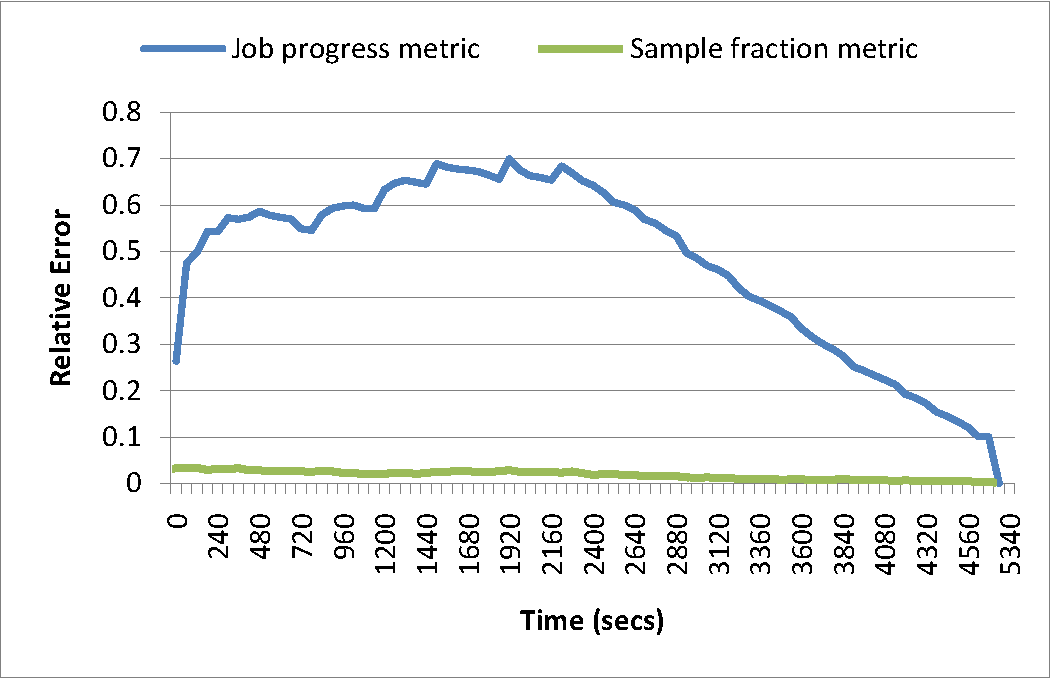
\includegraphics[width=0.48\linewidth]{eval/aprx-click-hour.pdf}}
  \hspace{4pt}
  \subfloat[][Example approximate answer]{\label{fig:approx-hour}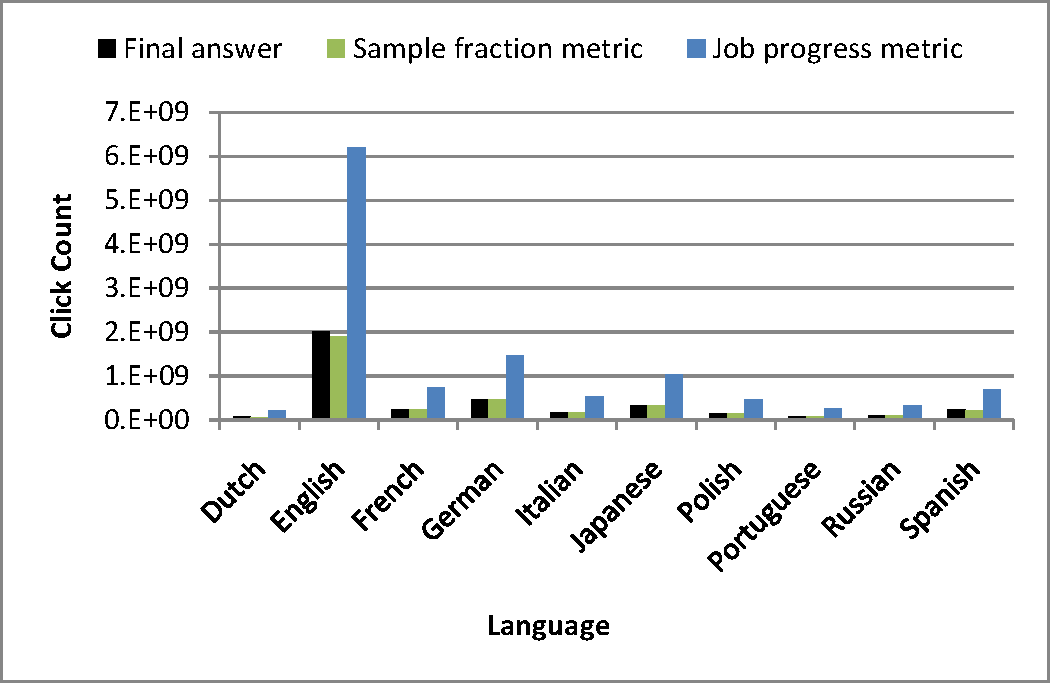
\includegraphics[width=0.48\linewidth]{eval/aprx-click-hour-actual.pdf}}
  \caption{Comparison of two approximation metrics. 
    Figure~\subref{fig:approx-relative} shows the relative error for
    each approximation metric over the runtime of the job, averaged over all
    groups. Figure~\subref{fig:approx-hour} compares an example approximate
    answer produced by each metric with the final answer, for each language and
    for a single hour.}
\label{fig:approx}
\end{figure*}

In our second experiment, we considered the effectiveness of the job progress
metric described in Section~\ref{sec:online-metric}. Unsurprisingly, this metric
can be inaccurate when it is used to estimate the accuracy of the approximate
answers produced by online aggregation. In this experiment, we compared the job
progress metric with a simple user-defined metric that leverages knowledge of
the query and data set. HOP allows such metrics, although developing such a
custom metric imposes more burden on the programmer than using the generic
progress-based metric.

We used a data set containing seven months of hourly page view statistics for
more than 2.5 million Wikipedia articles~\cite{wikistats}. This constituted
320GB of compressed data (1TB uncompressed), divided into 5066 compressed
files. We stored the data set on HDFS and assigned a single map task to each
file, which was decompressed before the map function was applied.

We wrote a MapReduce job to count the total number of page views for each
language and each hour of the day. In other words, our query grouped by language
and hour of day, and summed the number of page views that occurred in each
group. To enable more accurate approximate answers, we modified the map function
to include the fraction of a given hour that each record represents. The reduce
function summed these fractions for a given hour, which equated to one for all
records from a single map task. Since the total number of hours was known ahead
of time, we could use the result of this sum over all map outputs to determine
the total fraction of each hour that had been sampled. We call this user-defined
metric the ``sample fraction.''

To compute approximate answers, each intermediate result was scaled up using two
different metrics: the generic metric based on job progress and the sample
fraction described above. Figure~\ref{fig:approx-relative} reports the relative
error of the two metrics, averaged over all groups. Figure~\ref{fig:approx-hour}
shows an example approximate answer for a single hour using both metrics
(computed two minutes into the job runtime). This figure also contains the final
answer for comparison. Both results indicate that the sample fraction metric provides a
much more accurate approximate answer for this query than the progress-based
metric.

Job progress is clearly the wrong metric to use for approximating the final
answer of this query. The primary reason is that it is too coarse of a
metric. Each intermediate result was computed from some fraction of each
hour. However, the job progress assumes that this fraction is uniform across all
hours, when in fact we could have received much more of one hour and much less
of another. This assumption of uniformity in the job progress resulted in a
significant approximation error. By contrast, the sample fraction scales the
approximate answer for each group according to the actual fraction of data seen for
that group, yielding much more accurate approximations.

\section{Continuous Queries}
\label{sec:continuous}

MapReduce is often used to analyze streams of constantly-arriving
data, such as URL access logs~\cite{mapreduce-osdi} and system console
logs~\cite{sosp-mining}. Because of traditional constraints on MapReduce, this 
is done in large batches that can only provide periodic views of activity.
This introduces
significant latency into a data analysis process that ideally should run in 
near-real time. It is also
potentially inefficient: each new MapReduce job does not have access
to the computational state of the last analysis run, so this state
must be recomputed from scratch. The programmer can manually save the
state of each job and then reload it for the next analysis operation,
but this is labor-intensive.

Our pipelined version of Hadoop allows an alternative architecture:
MapReduce jobs that run \emph{continuously}, accepting new data as it
becomes available and analyzing it immediately. This allows for near-real-time
analysis of data streams, and thus
allows the MapReduce programming model to be applied to domains such
as environment monitoring and real-time fraud detection.

In this section, we describe how HOP supports continuous MapReduce
jobs, and how we used this feature to implement a rudimentary
cluster monitoring tool.

\subsection{Continuous MapReduce Jobs}
A bare-bones implementation of continuous MapReduce jobs is easy to
implement using pipelining. No changes are needed to implement
continuous map tasks: map output is already delivered to the
appropriate reduce task shortly after it is generated. We added an
optional ``flush'' API that allows map functions to force their current
output to reduce tasks. When a reduce task is unable to accept such data, the mapper framework
stores it locally and sends it at a later time. 
With proper scheduling of reducers, this API allows a map task to ensure that an output record is promptly sent to the appropriate
reducer.

To support continuous reduce tasks, the user-defined reduce function
must be periodically invoked on the map output available at that
reducer. Applications will have different requirements for how
frequently the reduce function should be invoked; possible choices
include periods based on wall-clock time, logical time (e.g., the
value of a field in the map task output), and the number of input rows
delivered to the reducer. The output of the reduce function can be
written to HDFS, as in our implementation of online
aggregation. However, other choices are possible; our prototype system
monitoring application (described below) sends an alert via email if
an anomalous situation is detected.

In our current implementation, the number of map and reduce tasks is
fixed, and must be configured by the user. This is clearly
problematic: manual configuration is error-prone, and many stream
processing applications exhibit ``bursty'' traffic patterns, in which
peak load far exceeds average load. In the future, we plan to add
support for elastic scaleup/scaledown of map and reduce tasks in
response to variations in load.

\subsubsection{Fault Tolerance}
In the checkpoint/restart fault-tolerance model used by Hadoop, mappers retain
their output until the end of the job to facilitate fast recovery from reducer
failures. In a continuous query context, this is infeasible, since mapper
history is in principle unbounded.  However, many continuous reduce functions
(e.g., 30-second moving average) only require a suffix of the map output stream.
This common case can be supported easily, by extending the \JT\ interface to
capture a rolling notion of reducer consumption.  Map-side spill files are
maintained in a ring buffer with unique IDs for spill files over time. When a
reducer commits an output to HDFS, it informs the \JT\ about the \emph{run} of
map output records it no longer needs, identifying the run by spill file IDs and
offsets within those files.  The \JT\ can then tell mappers to garbage collect
the appropriate data.

In principle, complex reducers may depend on very long (or infinite) histories of map records to accurately reconstruct their internal state.  In that case, deleting spill files
from the map-side ring buffer will result in potentially inaccurate recovery after faults.  Such scenarios can be handled by having reducers checkpoint internal state to HDFS, along with markers for the mapper offsets at which the internal state was checkpointed.  The MapReduce framework can be extended with APIs to help with state serialization and offset management, but it still presents a programming burden on the user to correctly identify the sensitive internal state.  That burden can be avoided by more heavyweight process-pair 
techniques for fault tolerance, but those are quite complex and use significant resources~\cite{flux-ft}.  In our work to date we have focused on cases where reducers can be recovered from a reasonable-sized history at the mappers, favoring minor extensions to the simple fault-tolerance approach used in Hadoop.

\subsection{Prototype Monitoring System}
Our monitoring system is composed of \emph{agents} that run on each monitored
machine and record statistics of interest (e.g., load average, I/O operations
per second, etc.). Each agent is implemented as a continuous map task: rather
than reading from HDFS, the map task instead reads from various system-local
data streams (e.g., \texttt{/proc}).

Each agent forwards statistics to an \emph{aggregator} that is implemented as a
continuous reduce task. The aggregator records how agent-local statistics evolve
over time (e.g., by computing windowed-averages), and compares statistics
between agents to detect anomalous behavior. Each aggregator monitors the agents
that report to it, but might also report statistical summaries to another
``upstream'' aggregator. For example, the system might be configured to have an
aggregator for each rack and then a second level of aggregators that compare
statistics between racks to analyze datacenter-wide behavior.

\subsection{Evaluation}
\begin{figure}[t]
%%\begin{minipage}{0.5\linewidth}
  \centering
  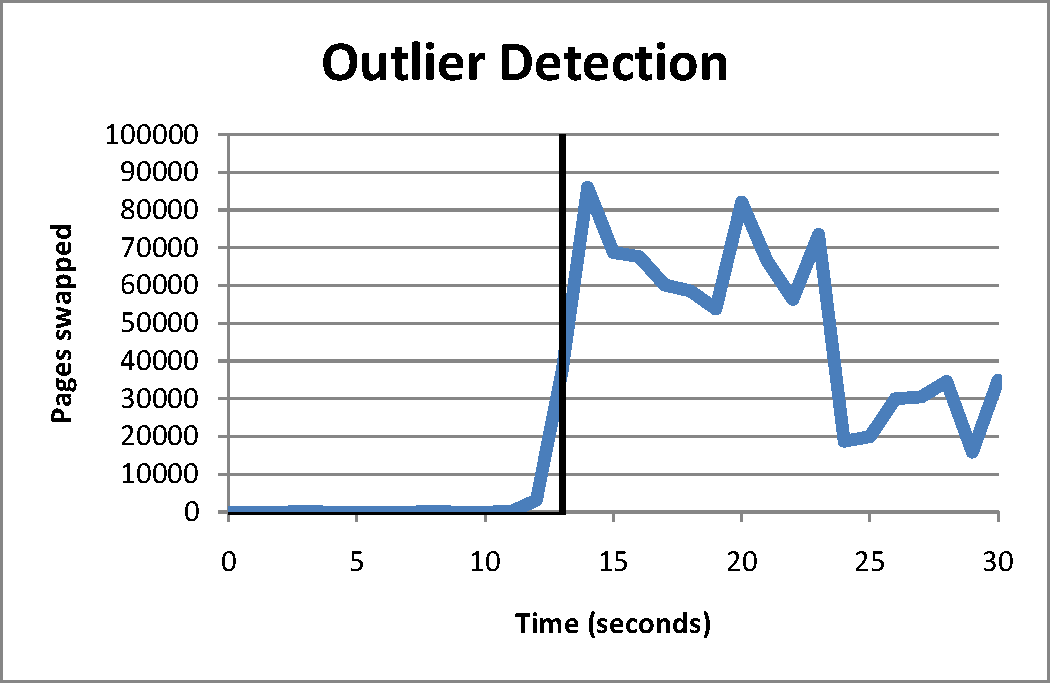
\includegraphics[width=0.95\linewidth]{eval/continue.pdf}
%%\end{minipage}
  \caption{Number of pages swapped over time on the thrashing host, as reported
    by \texttt{vmstat}.  The vertical line indicates the time at which the alert
    was sent by the monitoring system.}
\label{fig:outlier}
\end{figure}

To validate our prototype system monitoring tool, we constructed a
scenario in which one member of a MapReduce cluster begins thrashing
during the execution of a job. Our goal was to test how quickly our
monitoring system would detect this behavior. The basic mechanism is
similar to an alert system one of the authors implemented at an
Internet search company.

We used a simple load metric (a linear combination of CPU utilization,
paging, and swap activity). The continuous reduce function maintains
windows over samples of this metric: at regular intervals, it
compares the 20 second moving average of the load metric for each host
to the 120 second moving average of all the hosts in the cluster
\emph{except} that host.  If the given host's load metric is more
than two standard deviations above the global average, it is
considered an outlier and a tentative alert is issued.  To dampen
false positives in ``bursty'' load scenarios, we do not issue an alert
until we have received 10 tentative alerts within a time window.

We deployed this system on an EC2 cluster consisting of 7 ``large''
nodes (large nodes were chosen because EC2 allocates an entire
physical host machine to them). We ran a wordcount job on the 5.5GB Wikipedia
data set, using 5 map tasks and 2 reduce tasks (1 task per host). After
the job had been running for about 10 seconds, we selected a node
running a task and launched a program that induced thrashing.

We report detection latency in Figure~\ref{fig:outlier}. The vertical bar
indicates the time at which the monitoring tool fired a (non-tentative)
alert. The thrashing host was detected very rapidly---notably faster than the
5-second {\TT}-{\JT} heartbeat cycle that is used to detect straggler tasks in
stock Hadoop. We envision using these alerts to do early detection of stragglers
within a MapReduce job: HOP could make scheduling decisions for a job by running
a secondary continuous monitoring query. Compared to out-of-band monitoring
tools, this economy of mechanism---reusing the MapReduce infrastructure for
reflective monitoring---has benefits in software maintenance and system
management.

\begin{figure*}[t]
\begin{minipage}{0.5\linewidth}
  \centering
        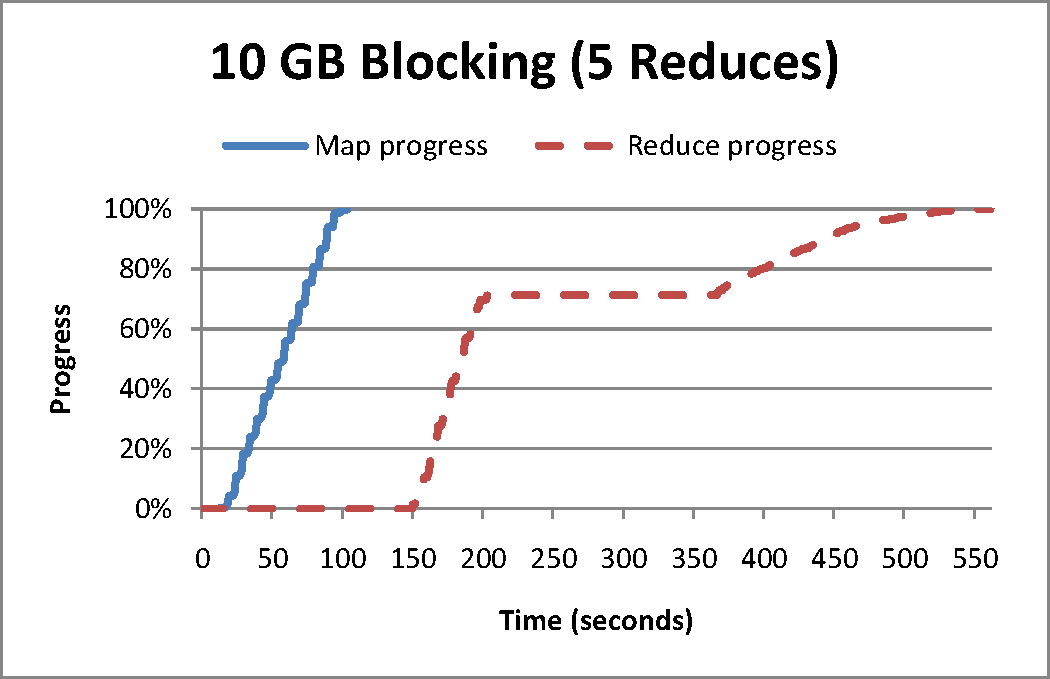
\includegraphics[width=0.90\linewidth]{eval/wc_10gb_20m5r_blocking}
\end{minipage}
\begin{minipage}{0.5\linewidth}
  \centering
        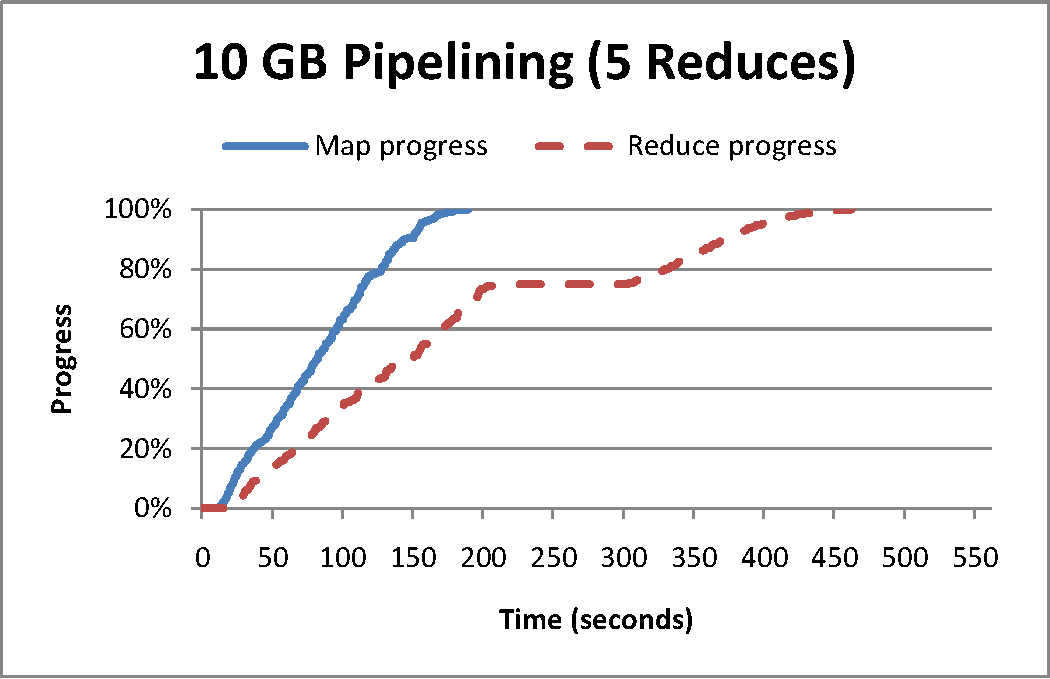
\includegraphics[width=0.90\linewidth]{eval/wc_10gb_20m5r_pipeline}
\end{minipage}
\caption{CDF of map and reduce task completion times for a 10GB wordcount job
  using 20 map tasks and 5 reduce tasks (512MB block size). The total job
  runtimes were 561 seconds for blocking and 462 seconds for pipelining.}
\label{fig:wc1}
\vspace{-4pt}
\end{figure*}

\begin{figure*}[t]
\begin{minipage}{0.5\linewidth}
  \centering
        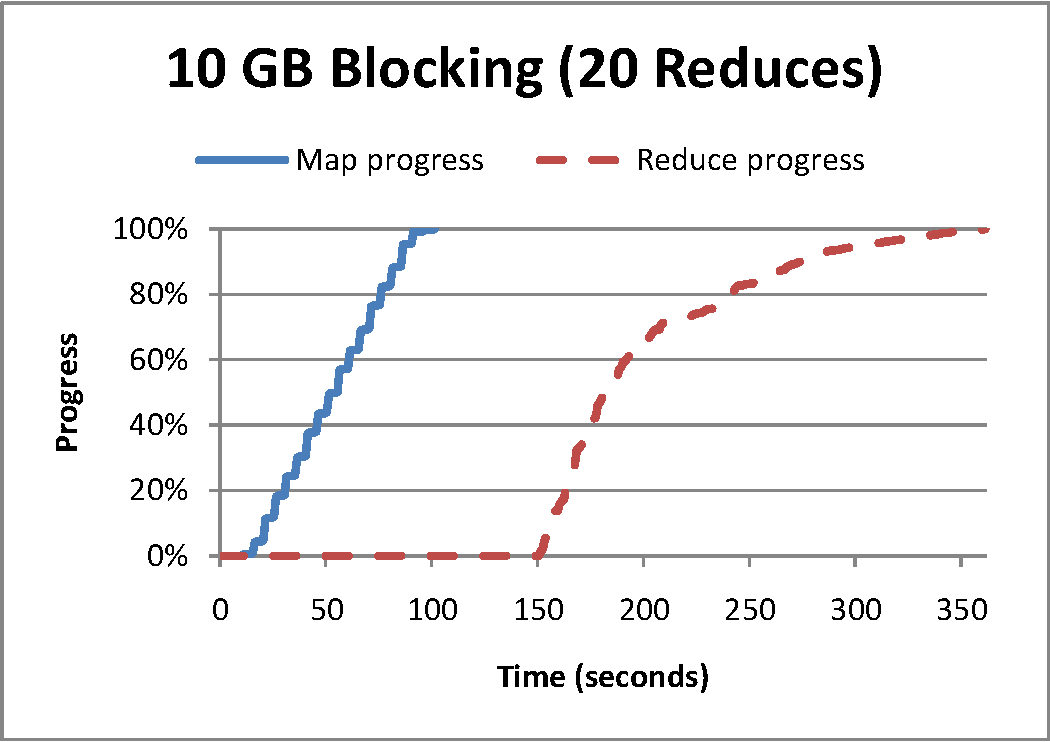
\includegraphics[width=0.88\linewidth]{eval/wc_10gb_20m20r_blocking}
\end{minipage}
\begin{minipage}{0.5\linewidth}
  \centering
        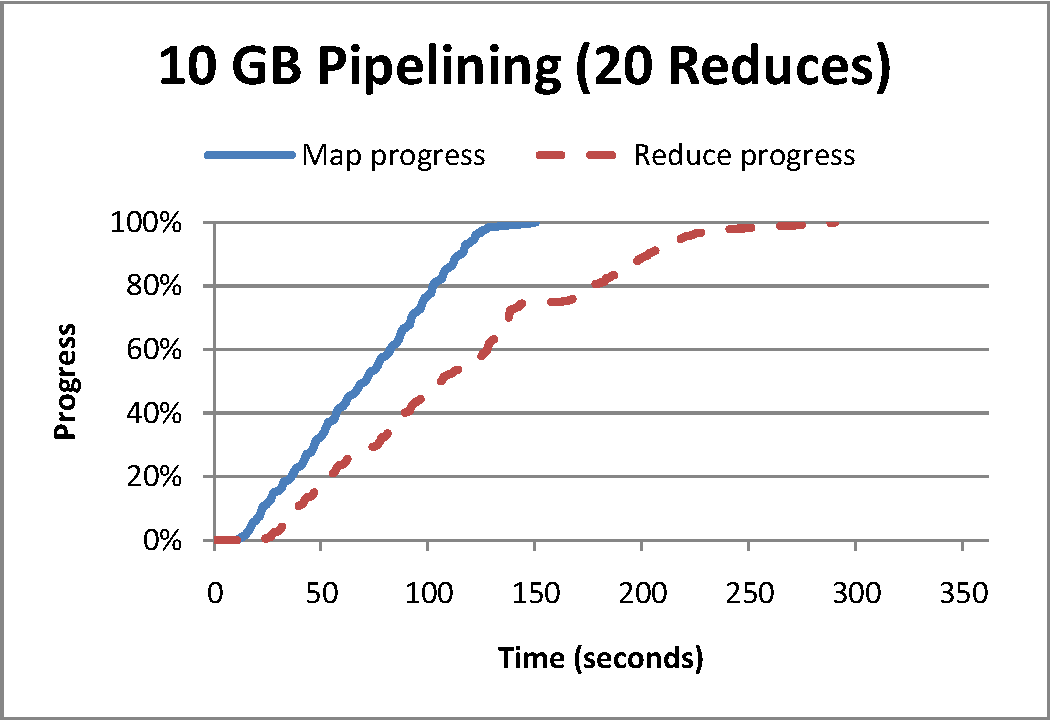
\includegraphics[width=0.90\linewidth]{eval/wc_10gb_20m20r_pipeline}
\end{minipage}
\caption{CDF of map and reduce task completion times for a 10GB wordcount job
  using 20 map tasks and 20 reduce tasks (512MB block size). The total job
  runtimes were 361 seconds for blocking and 290 seconds for pipelining.}
\label{fig:wc2}
\vspace{-4pt}
\end{figure*}

\begin{figure*}[t]
\begin{minipage}{0.5\linewidth}
  \centering
        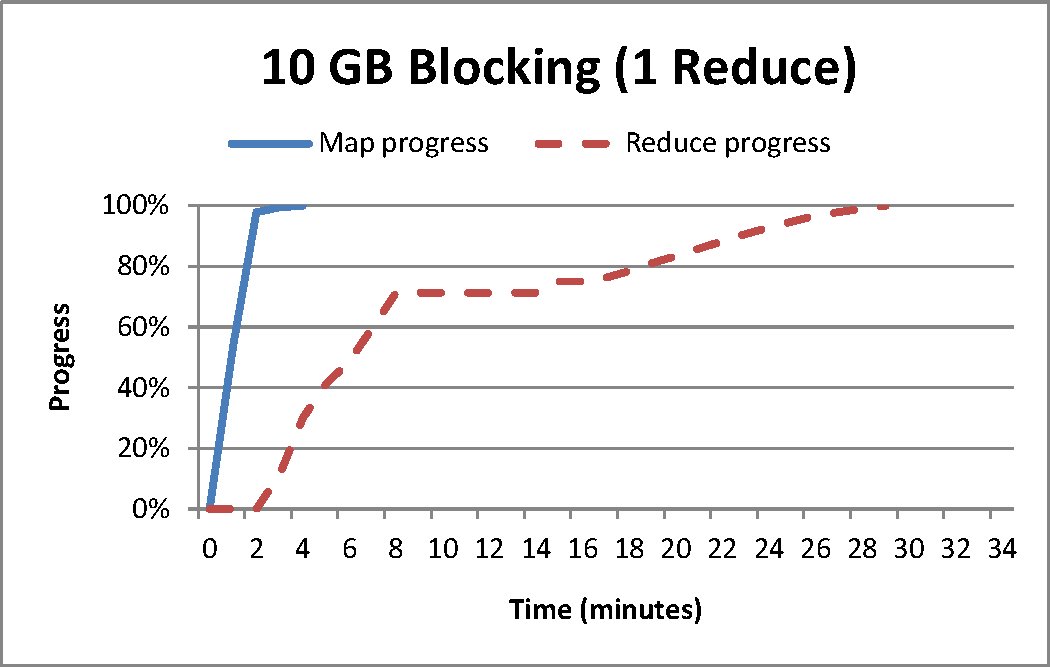
\includegraphics[width=0.95\linewidth]{eval/wc_10gb_20m1r_blocking}
\end{minipage}
\begin{minipage}{0.5\linewidth}
  \centering
        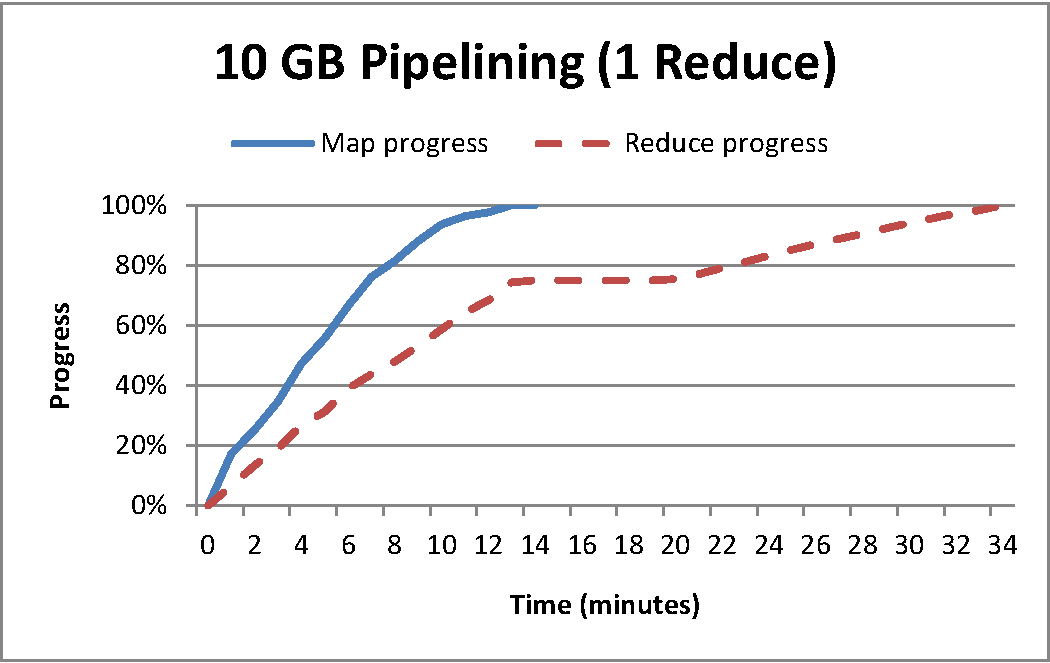
\includegraphics[width=0.95\linewidth]{eval/wc_10gb_20m1r_pipeline}
\end{minipage}
\caption{CDF of map and reduce task completion times for a 10GB wordcount job
  using 20 map tasks and 1 reduce task (512MB block size). The total job
  runtimes were 29 minutes for blocking and 34 minutes for pipelining.}
\label{fig:wc3}
\vspace{-4pt}
\end{figure*}

\section{Performance Evaluation}
\label{sec:perf}

A thorough performance comparison between pipelining and blocking is beyond the
scope of this paper. In this section, we instead demonstrate that pipelining can
reduce job completion times in some configurations.

We report performance using both large (512MB) and small (32MB) HDFS block sizes
using a single workload (a wordcount job over randomly-generated text). Since
the words were generated using a uniform distribution, map-side combiners were
ineffective for this workload. We performed all experiments using relatively
small clusters of Amazon EC2 nodes. We also did not consider performance in an
environment where multiple concurrent jobs are executing simultaneously.

\begin{figure*}[t]
\begin{minipage}{0.5\linewidth}
  \centering
        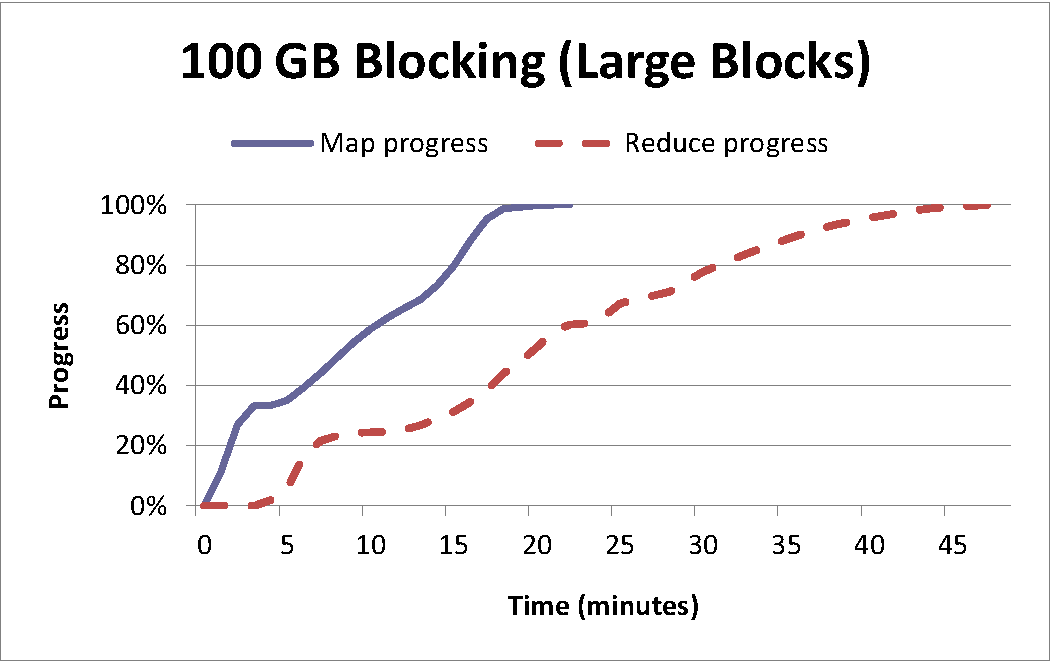
\includegraphics[width=0.95\linewidth]{eval/wc_100gb_240m60r_blocking}
\end{minipage}
\begin{minipage}{0.5\linewidth}
  \centering
        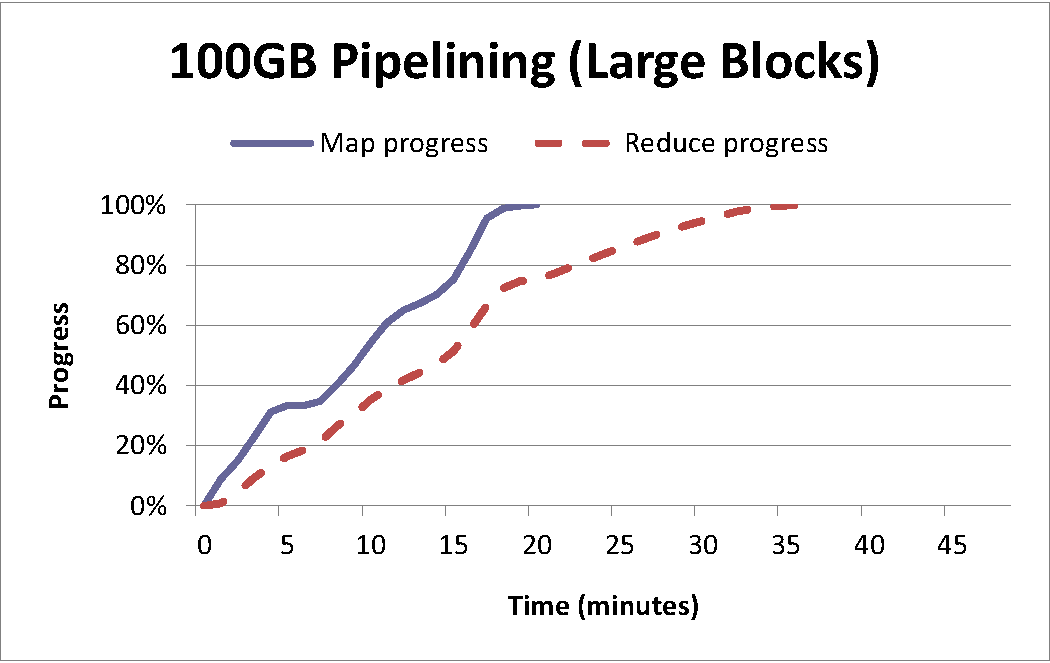
\includegraphics[width=0.95\linewidth]{eval/wc_100gb_240m60r_pipeline}
\end{minipage}
\caption{CDF of map and reduce task completion times for a 100GB wordcount job
  using 240 map tasks and 60 reduce tasks (512MB block size). The total job
  runtimes were 48 minutes for blocking and 36 minutes for pipelining.}
\label{fig:wc4}
\end{figure*}

\begin{figure*}[t]
\begin{minipage}{0.5\linewidth}
  \centering
        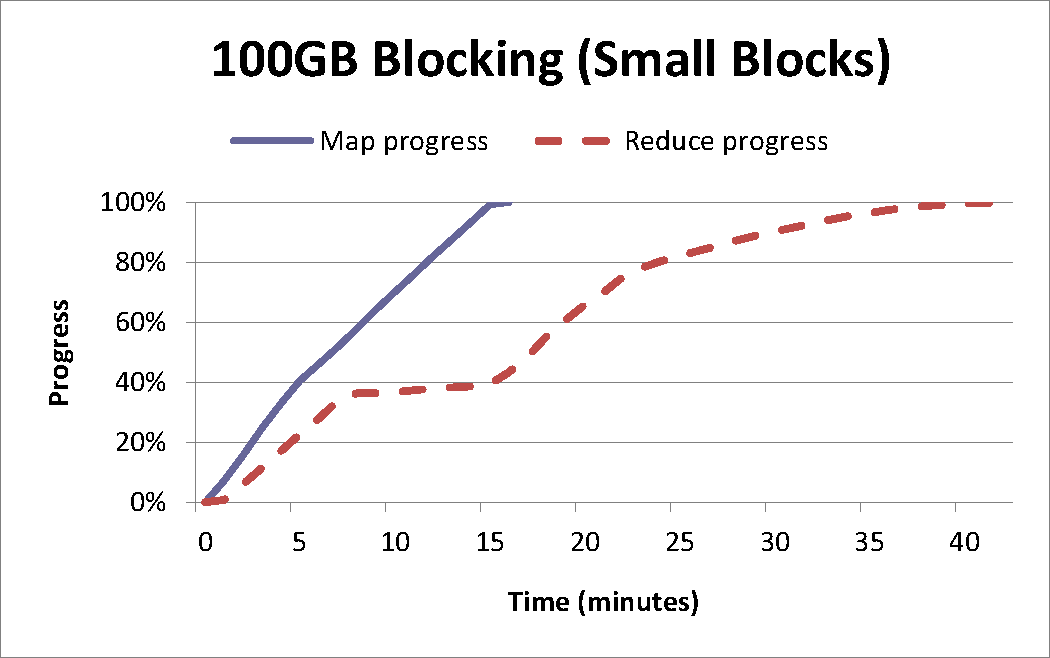
\includegraphics[width=0.95\linewidth]{eval/wc_100gb_3120m60r_blocking}
\end{minipage}
\begin{minipage}{0.5\linewidth}
  \centering
        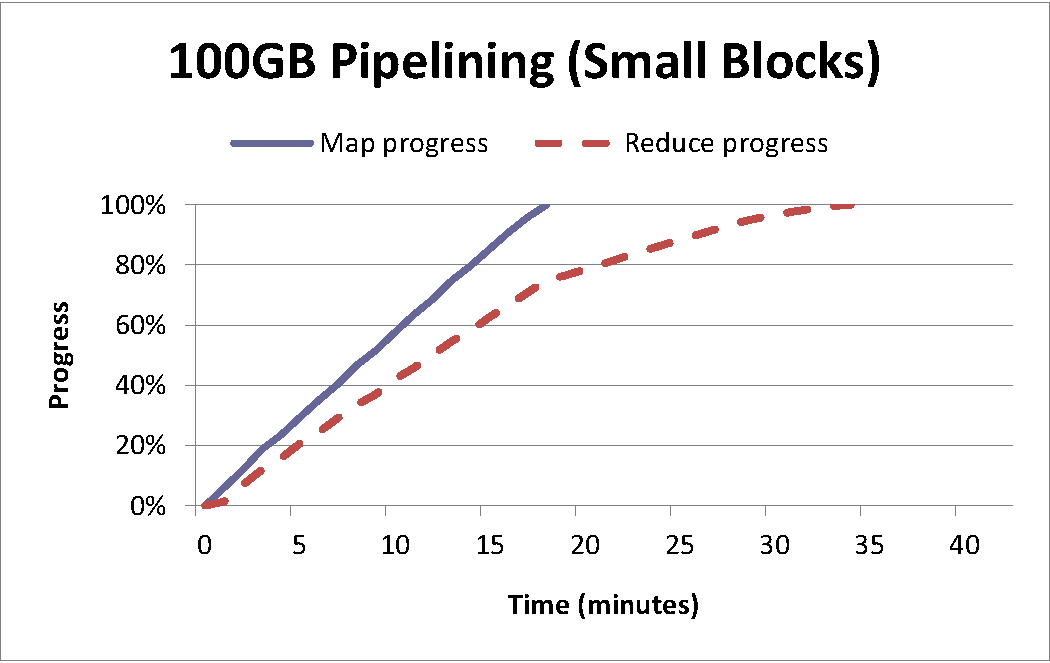
\includegraphics[width=0.95\linewidth]{eval/wc_100gb_3120m60r_pipeline}
\end{minipage}
\caption{CDF of map and reduce task completion times for a 100GB wordcount job
  using 3120 map tasks and 60 reduce tasks (32MB block size). The total job
  runtimes were 42 minutes for blocking and 34 minutes for pipelining.}
\label{fig:wc5}
\end{figure*}

\subsection{Background and Configuration}
Before diving into the performance experiments, it is important to further
describe the division of labor in a HOP job, which is broken into task phases. A
map task consists of two work phases: {\em map} and {\em sort}. The majority
of work is performed in the {\em map} phase, where the map function is applied
to each record in the input and subsequently sent to an output buffer.  Once the
entire input has been processed, the map task enters the {\em sort} phase, where
a final merge sort of all intermediate spill files is performed before
registering the final output with the \TT. The progress reported by a map task
corresponds to the {\em map} phase only.

A reduce task in HOP is divided into three work phases: {\em shuffle}, {\em
  reduce}, and {\em commit}.  In the {\em shuffle} phase, reduce tasks receive
their portion of the output from each map.  In HOP, the {\em shuffle} phase
consumes 75\% of the overall reduce task progress while the remaining 25\% is
allocated to the {\em reduce} and {\em commit} phase.\footnote{The stock version
  of Hadoop divides the reduce progress evenly among the three phases. We
  deviated from this approach because we wanted to focus more on the progress
  during the {\em shuffle} phase.}  In the {\em shuffle} phase, reduce tasks
periodically perform a merge sort on the already received map output. These
intermediate merge sorts decrease the amount of sorting work performed at the
end of the {\em shuffle} phase. After receiving its portion of data from all map
tasks, the reduce task performs a final merge sort and enters the {\em reduce}
phase.

By pushing work from map tasks to reduce tasks more aggressively, pipelining can
enable better overlapping of map and reduce computation, especially when the
node on which a reduce task is scheduled would otherwise be
underutilized. However, when reduce tasks are already the bottleneck, pipelining
offers fewer performance benefits, and may even hurt performance by placing
additional load on the reduce nodes.

The {\em sort} phase in the map task minimizes the merging work that reduce
tasks must perform at the end of the {\em shuffle} phase. When pipelining is
enabled, the {\em sort} phase is avoided since map tasks have already sent some
fraction of the spill files to concurrently running reduce tasks. Therefore,
pipelining increases the merging workload placed on the reducer. The adaptive
pipelining scheme described in Section~\ref{sec:mapout} attempts to ensure that
reduce tasks are not overwhelmed with additional load.

We used two Amazon EC2 clusters depending on the size of the experiment:
``small'' jobs used 10 worker nodes, while ``large'' jobs used 20. Each node
was an ``extra large'' EC2 instances with 15GB of memory and four virtual cores.

\subsection{Small Job Results}
Our first experiment focused on the performance of small jobs in an
underutilized cluster. We ran a 10GB wordcount with a 512MB block size, yielding
20 map tasks. We used 10 worker nodes and configured each worker to execute at
most two map and two reduce tasks simultaneously. We ran several experiments to
compare the performance of blocking and pipelining using different numbers of
reduce tasks.

Figure~\ref{fig:wc1} reports the results with five reduce tasks. A plateau can
be seen at 75\% progress for both blocking and pipelining. At this point in the
job, all reduce tasks have completed the {\em shuffle} phase; the plateau is
caused by the time taken to perform a final merge of all map output before
entering the {\em reduce} phase. Notice that the plateau for the pipelining case
is shorter. With pipelining, reduce tasks receive map outputs earlier and can
begin sorting earlier, thereby reducing the time required for the final merge.

Figure~\ref{fig:wc2} reports the results with twenty reduce tasks. Using more
reduce tasks decreases the amount of merging that any one reduce task must
perform, which reduces the duration of the plateau at 75\% progress. In the
blocking case, the plateau is practically gone.%  However, with pipelining we
% still see a small plateau at 75\%, which means that the final sort spilled to
% disk. Since the combiner is not executed on the full map output, pipelining can
% add extra memory pressure over blocking. That extra memory pressure for this
% experiment was not enough slow pipelining down over blocking. However, a job
% that contains a more effective combiner may be better executed in blocking
% mode.

Note that in both experiments, the map phase finishes faster with blocking than
with pipelining. This is because pipelining allows reduce tasks to begin
executing more quickly; hence, the reduce tasks compete for resources with the
map tasks, causing the map phase to take slightly longer. In this case, the
increase in map duration is outweighed by the increase in cluster utilization,
resulting in shorter job completion times: pipelining reduced completion time by
17.7\% with 5 reducers and by 19.7\% with 20 reducers.

Figure~\ref{fig:wc3} describes an experiment in which we ran a 10GB wordcount
job using a single reduce task. This caused job completion times to increase
dramatically for both pipelining and blocking, because of the extreme load
placed on the reduce node. Pipelining delayed job completion by
\texttildelow{}17\%, which suggests that our simple adaptive flow control scheme
(Section~\ref{sec:mapout}) was unable to move load back to the map tasks
aggressively enough.

\subsection{Large Job Results}
Our second set of experiments focused on the performance of somewhat larger
jobs. We increased the input size to 100GB (from 10GB) and the number of worker
nodes to 20 (from 10). Each worker was configured to execute at most four map
and three reduce tasks, which meant that at most 80 map and 60 reduce tasks
could execute at once. We conducted two sets of experimental runs, each run
comparing blocking to pipelining using either large (512MB) or small (32MB)
block sizes. We were interested in blocking performance with small block sizes
because blocking can effectively emulate pipelining if the block size is small
enough.

Figure~\ref{fig:wc4} reports the performance of a 100GB wordcount job with 512MB
blocks, which resulted in 240 map tasks, scheduled in three waves of 80 tasks
each. The 60 reduce tasks were coscheduled with the first wave of map tasks. In
the blocking case, the reduce tasks began working as soon as they received the
output of the first wave, which is why the reduce progress begins to climb
around four minutes (well before the completion of all maps). Pipelining was
able to achieve significantly better cluster utilization, and hence reduced job
completion time by \texttildelow{}25\%.

% Comparing the reduce progress in blocking to pipelining, we see that reduce
% tasks make more progress during the {\em shuffle} phase when pipelining is
% enabled. What is even more interesting is that the {\em reduce} phase is also
% shorter in the case of pipelining. The reason for this is subtle; all reduce
% tasks enter the {\em phase} around the same time since data is shipped in
% smaller increments. In the blocking case, when the final wave of map tasks
% finish they all try to send the entire output to reduce tasks at the same time,
% which increases the variance on receiving the complete output from all map
% tasks. That is, some reduce tasks enter the {\em reduce} phase well in advance
% of others.

Figure~\ref{fig:wc5} reports the performance of blocking and pipelining using
32MB blocks. While the performance of pipelining remained similar, the
performance of blocking improved considerably, but still trailed somewhat behind
pipelining. Using block sizes smaller than 32MB did not yield a significant
performance improvement in our experiments.

% \subsection{Discussion}

% As mentioned before, a complete performance evaluation is beyond the scope for this paper and we leave
% such a study for future work. The focus here was to provide some initial insight into the performance benefits
% of pipelining. We also wanted to evaluate the adaptive policy of our pipelining scheme. To this end, we
% found such a policy paramount in discovering the right amount of pipelining to perform based on runtime
% factors; network capacity and reduce task (consumer) load.

%\begin{figure*}[t]
%\begin{minipage}{0.5\linewidth}
%        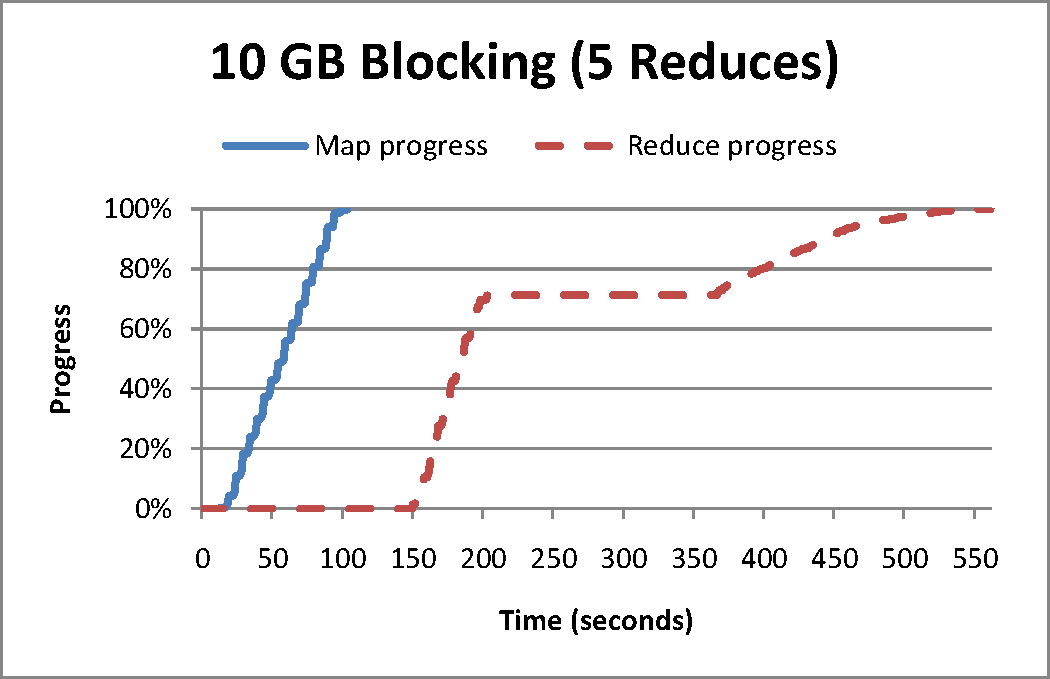
\includegraphics[width=0.95\linewidth]{eval/wc_10gb_20m5r_blocking}
%\end{minipage}
%\begin{minipage}{0.5\linewidth}
%        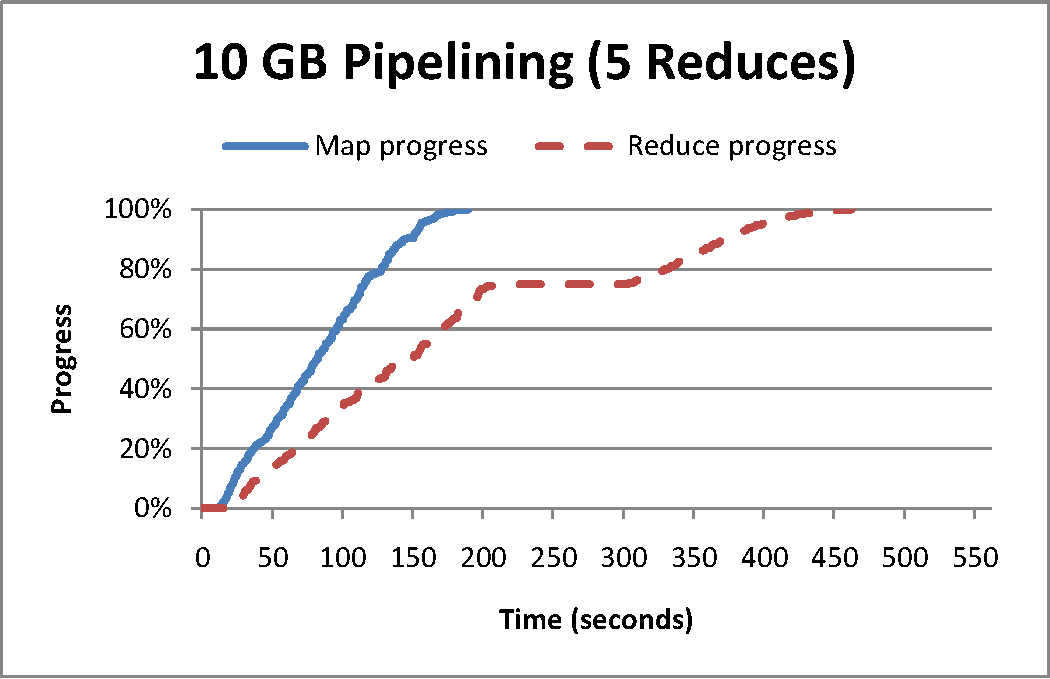
\includegraphics[width=0.95\linewidth]{eval/wc_10gb_20m5r_pipeline}
%\end{minipage}
%\caption{CDF of map and reduce task completion times for a sort job on
%  5.5GB of text extracted from Wikipedia. The total job runtimes were
%  927 seconds for blocking, and 610 seconds for pipelining.}
%\label{fig:sort}
%\end{figure*}

%We conducted a series of performance experiments using a 60-node
%cluster on Amazon EC2. One node executed the Hadoop \JT\ and the HDFS
%\NN, while the remaining 59 nodes served as slaves for running the
%{\TT}s and HDFS {\DN}s. All nodes executed on ``high-CPU medium'' EC2
%instances with 1.7GB of memory and two virtual cores. Each virtual
%core is the equivalent of a 2007-era 2.5Ghz Intel Xeon processor.

%We began by measuring the performance of a simple MapReduce job that
%does not use a combiner. Sorting is commonly used as a benchmark for
%basic MapReduce performance, because of the implicit sort done by the
%reduce phase. We sorted 5.5GB of article text extracted from
%Wikipedia; each word from the text was parsed as a separate
%record. Figure~\ref{fig:sort} describes sort performance on the EC2
%cluster using an HDFS block size of 128MB (yielding 40 map tasks). We
%configured the system to use 59 reducers. In each graph, we give the
%CDF of map and reduce task completion. The left and right graphs
%depict blocking and pipelined performance, respectively.

%Pipelining dominates blocking for this configuration, in part because
%it achieves better cluster utilization: the reduce tasks in the
%blocking job were idle for the first $192$ seconds of the experiment,
%whereas for the pipelined job, reducers began doing useful work within
%$20$ seconds. Note that in a highly-utilized cluster, increased
%pipeline parallelism would not necessarily lead to an improvement in
%total throughput. However, these results suggest that pipelining can
%substantially reduce the response time of an individual job, which can
%often be important (e.g., quickly executing high-priority jobs).

\section{Related Work}
\label{sec:relwork}
The shopping cart case study in Section~\ref{sec:case} was motivated by the
Amazon Dynamo paper~\cite{dynamo}, as well as the related discussion by Helland
and Campbell~\cite{quicksand}. Systems with loose consistency requirements have
been explored in depth by both the systems and database management communities
(e.g.,~\cite{sagas,leases,dangers,bayou}); we do not attempt to provide
an exhaustive survey here.

The Bloom language is inspired by earlier work that attempts to integrate
databases and programming languages.  This includes early research such as
Gem~\cite{gem} and more recent object-relational mapping layers like Ruby on
Rails.  Unlike these efforts, Bloom is targeted at the development of both
distributed infrastructure and distributed applications, so it does not make any
assumptions about the presence of a database system ``underneath it.''  Given
our prototype implementation in Ruby, it is tempting to integrate Bud with
Rails; we have left this for future work.

Our work on Bloom bears a resemblance to the Reactor
language~\cite{reactors}. Both languages target distributed programming and are
grounded in Datalog. Moreover, both languages combine declarative rules and
state into a single program construct. While Bloom uses a syntax inspired by
object-oriented languages, Reactor takes a more explicitly agent-oriented
approach. Reactor also includes synchronous coupling between agents as a
primitive; we have opted to only include asynchronous communication as a
language primitive and to provide synchronous coordination between nodes as a
library. Another significant different is that, like many rule-based languages,
Reactor includes some imperative constructs (e.g., \ldots), whereas rules in
Bloom are purely declarative.

Another recent language related to our work is Coherence~\cite{coherence}, which
also embraces ``disorderly'' programming. Unlike Bloom, Coherence is not
designed for distributed computing and is not based on logic programming.

There is a long history of attempts to design programming languages more
suitable to parallel and distributed systems; for example, Argus~\cite{argus}
and Linda~\cite{linda}.  Again, we do not hope to survey that literature here.
More pragmatically, Erlang is an oft-cited choice for distributed programming in
recent years.  Erlang's features and design style encourage the use of
asynchronous lightweight ``actors.''  As mentioned previously, we did a simple
Bloom prototype DSL in Erlang (which we cannot help but call ``Bloomerlang''),
and there is a natural correspondence between Bloom-style distributed rules and
Erlang actors.  However there is no requirement for Erlang programs to be
written in the disorderly style of Bloom. It is not obvious that typical Erlang
programs are significantly more amenable to a useful points-of-order analysis
than programs written in any other functional language.  For example, ordered
lists are basic constructs in functional languages, and without program
annotation or deeper analysis than we need to do in Bloom, any code that
modifies lists would need be marked as a point of order, much like our
destructive shopping cart.  We believe that Bloom's ``disorderly by default''
style encourages more disorderly programming; we know that its roots in database
theory bore fruit in terms of our analysis.  While we would be happy to see the
analysis ``ported'' to currently popular distributed programming environments,
it may be that design patterns using Bloom-esque disorderly programming are the
natural way to achieve this.

\section{Conclusion}
\label{sec:conclusion}
And thus, we conclude.

\section*{Acknowledgments}
We would like to thank Daniel Abadi, Kuang Chen, Mosharaf Chowdhury, Akshay
Krishnamurthy, Andrew Pavlo, Hong Tang , and our shepherd Jeff Dean for their
helpful comments and suggestions. This material is based upon work supported by
the National Science Foundation under Grant Nos.\ 0713661, 0722077 and 0803690,
the Air Force Office of Scientific Research under Grant No.\ FA95500810352, the
Natural Sciences and Engineering Research Council of Canada, and gifts from IBM,
Microsoft, and Yahoo!.

{\footnotesize \bibliographystyle{acm}
\bibliography{nsdi}}

\end{document}
